\section{Autoinducer analogues}

\subsection{HHQ derivative}

\subsubsection{Retrosynthesis of HHQ analogue \compound{cmpd:azHHQ}}

The retrosynthesis of HHQ analogue \compound{cmpd:azHHQ} is shown in \ref{sch:azHHQ_retro} and follows a synthesis devised by Baker\cite{Baker2014}. Octonyl chloride \compound{cmpd:OctoCl} can be converted to $\beta$-ketoester \compound{cmpd:bke} via a Meldrum's acid adduct. $\beta$-ketoester \compound{cmpd:bke} can be condensed with \textit{N}-Boc-\textit{p}-phenylenediamine \compound{cmpd:ambenboc} to form enamine \compound{cmpd:Bocenaman}, which can then be cyclised with polyphosphoric acid to form amino-HHQ \compound{cmpd:amHHQ}. The amine group of amino-HHQ \compound{cmpd:amHHQ} could be converted to a diazo group by reaction with \ce{NaNO2} and HCl, followed by displacement with \ce{NaN3} to form the final azido-HHQ product \compound{cmpd:azHHQ}\cite{Xu2013}.

\begin{scheme}[H]
	\begin{center}
		\schemeref[Mel]{cmpd:Mel}
		\schemeref[OctoCl]{cmpd:OctoCl}
		\schemeref[bke]{cmpd:bke}
		\schemeref[bket]{cmpd:bket}
		\schemeref[ambenboc]{cmpd:ambenboc}
		\schemeref[Bocenaman]{cmpd:Bocenaman}
		\schemeref[amHHQ]{cmpd:amHHQ}
		\schemeref[azHHQ]{cmpd:azHHQ}
		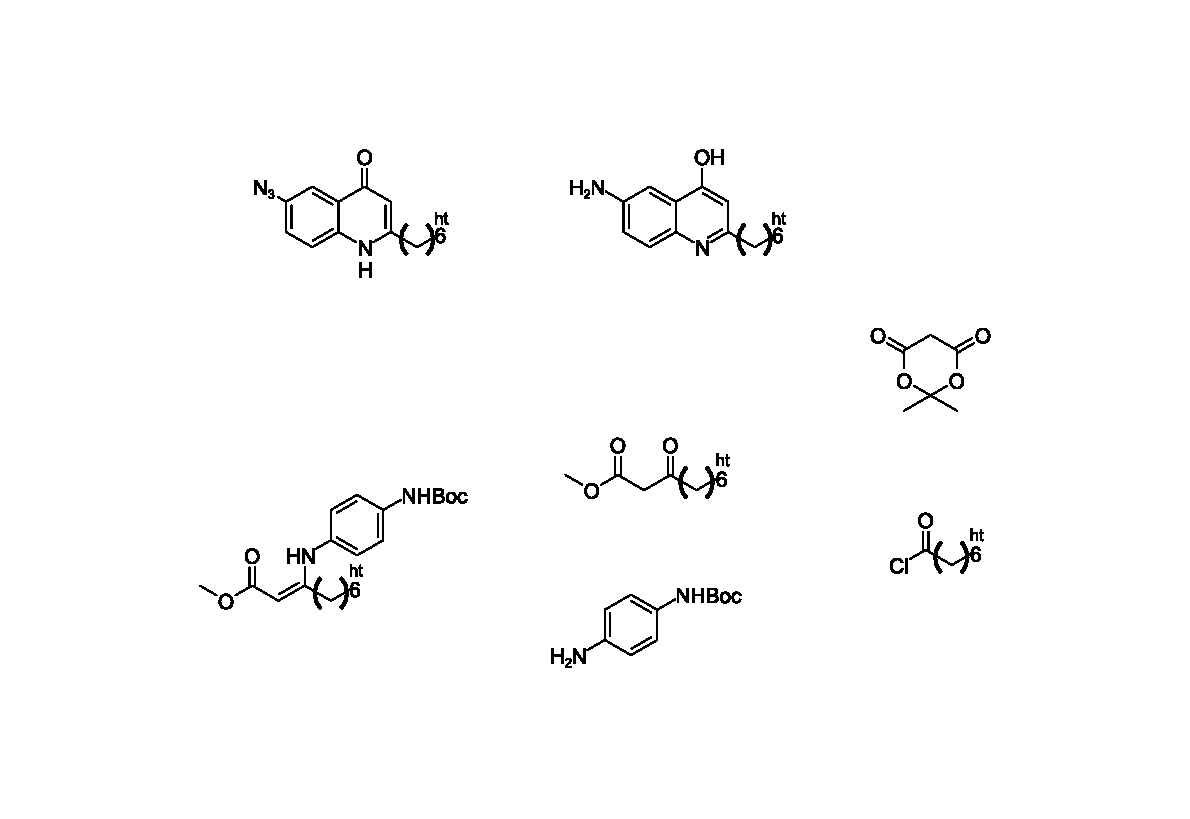
\includegraphics[width=\textwidth]{azHHQ_retro}
		\caption{The retrosynthesis of HHQ analogue \compound{cmpd:azHHQ}. 	
		\label{sch:azHHQ_retro}}
	\end{center}
\end{scheme}

\subsubsection{Synthesis of HHQ analogue \compound{cmpd:azHHQ} \label{sec:azHHQ}}

Amino-HHQ \compound{cmpd:amHHQ} was synthesised as shown in \ref{sch:azHHQ_synth} and follows the route devised by Baker\cite{Baker2014} described above.
The final step in the synthesis of \compound{cmpd:azHHQ} will be completed shortly.

\begin{scheme}[H]
	\begin{center}
		\schemeref[Mel]{cmpd:Mel}
		\schemeref[OctoCl]{cmpd:OctoCl}
		\schemeref[bke]{cmpd:bke}
		\schemeref[bket]{cmpd:bket}
		\schemeref[ambenboc]{cmpd:ambenboc}
		\schemeref[Bocenaman]{cmpd:Bocenaman}
		\schemeref[amHHQ]{cmpd:amHHQ}
		\schemeref[azHHQ]{cmpd:azHHQ}
		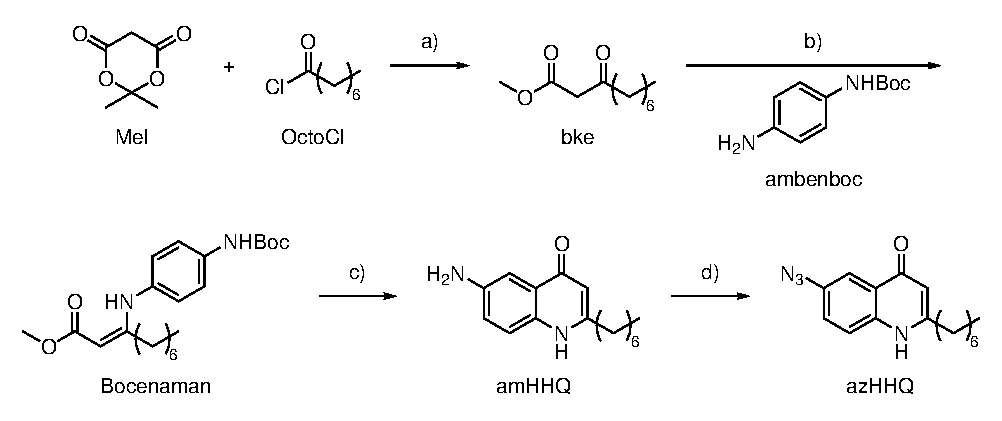
\includegraphics[width=\textwidth]{azHHQ_synth}
		\caption{The synthesis of \compound{cmpd:azHHQ}. 
		a) i) Pyridine, DCM, $0 ^{\circ}$C. ii) MeOH, reflux, 66 \% over two steps. 
		b) MeOH, reflux, 19 \%. 
		c) Polyphosphoric acid, $120 ^{\circ}$C, 72 \%. 
		d) i) \ce{NaNO2}, HCl, \ce{H2O}, 0 $^{\circ}$C. ii) \ce{NaN3}, \ce{H2O}, r.t. 
		\label{sch:azHHQ_synth}}
	\end{center}
\end{scheme}

\subsection{PQS derivative}

\subsubsection{Retrosynthesis of PQS derivative \compound{cmpd:azPQS}}

The retrosynthesis of PQS analogue \compound{cmpd:azPQS} is shown in \ref{sch:azPQS_retro}. The synthesis of 1-chlorononan-2-one \compound{cmpd:Clnon} from heptyl magnesium bromide \compound{cmpd:hepGr}\cite{Hodgkinson2012} and the Weinreb amide \compound{cmpd:ClWa}\cite{Hodgkinson2011} prepared from chloroacetyl chloride \compound{cmpd:ClAcCl} has been previously described by Hodgkinson \textit{et al.}\cite{Hodgkinson2012}. 
The synthesis of PQS described by Hodgkinson \textit{et al.}\cite{Hodgkinson2012} uses a microwave reaction of 1-chlorononan-2-one \compound{cmpd:Clnon} with anthranillic acid. It was hoped that the azide group could be installed by using 5-nitroanthranillic acid \compound{cmpd:5naa} in the place of anthranillic acid in this microwave reaction, so that the nitro group could then be converted to an azide group via an amine. However, the microwave-catalysed reaction fails when 5-nitroanthranillic acid \compound{cmpd:5naa} is used\cite{Baker2014}. Therefore, a two step process is employed instead. Firstly, ester \compound{cmpd:5naae} is formed by S$_N$2 displacement of the chlorine atom of 1-chlorononan-2-one \compound{cmpd:Clnon} by the carboxylate group of 5-nitroanthranillic \compound{cmpd:5naa}. The ester \compound{cmpd:5naae} is then cyclised using a polyphosphoric acid-catalysed reaction developed by Hradil \textit{et al.}\cite{Hradil1999} to form nitro-PQS \compound{cmpd:NPQS}. The nitro group can then be hydrogenated to form amino-PQS \compound{cmpd:amPQS} followed by conversion to azido-PQS \compound{cmpd:azPQS}\cite{Xu2013}.


\begin{scheme}[H]
	\begin{center}
		\schemeref[hepBr]{cmpd:hepBr}
		\schemeref[hepGr]{cmpd:hepGr}
		\schemeref[ClAcCl]{cmpd:ClAcCl}
		\schemeref[ClWa]{cmpd:ClWa}
		\schemeref[Clnon]{cmpd:Clnon}
		\schemeref[5naa]{cmpd:5naa}
		\schemeref[5naae]{cmpd:5naae}
		\schemeref[NPQS]{cmpd:NPQS}
		\schemeref[amPQS]{cmpd:amPQS}
		\schemeref[azPQS]{cmpd:azPQS}
		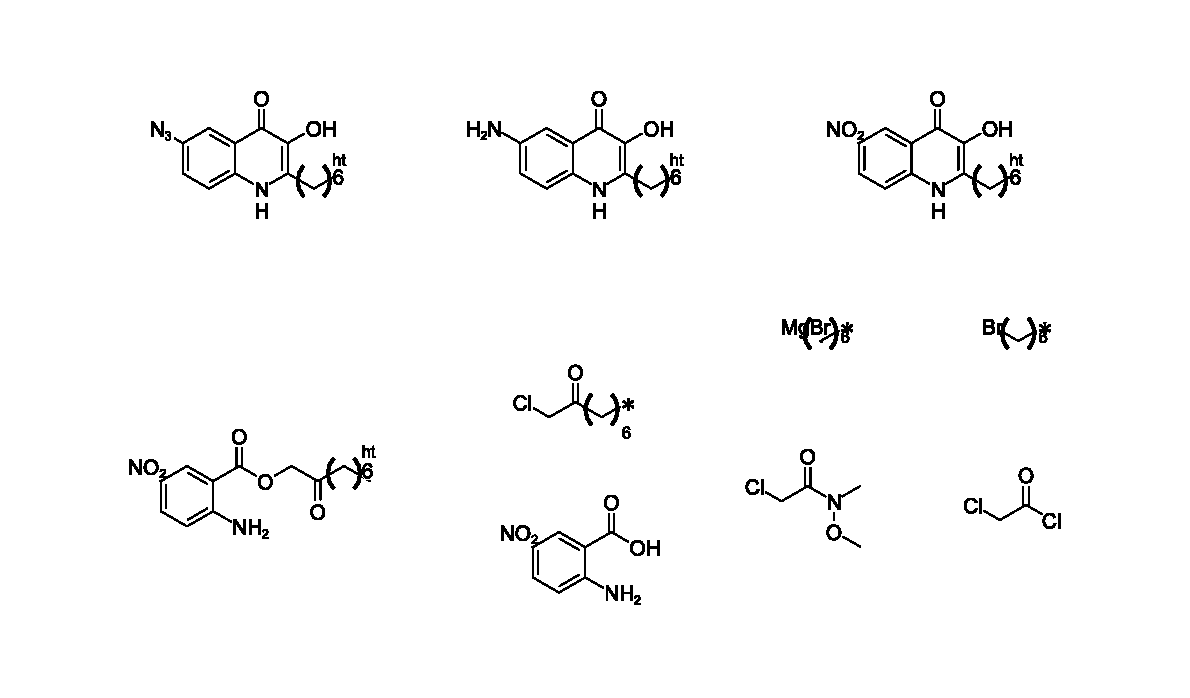
\includegraphics[width=\textwidth]{azPQS_retro}
		\caption{The retrosynthesis of PQS analogue \compound{cmpd:azPQS}. \label{sch:azPQS_retro}}
	\end{center}
\end{scheme}

\subsubsection{Synthesis of PQS derivative \compound{cmpd:azPQS}}

The Weinreb amide \compound{cmpd:ClWa} was prepared from chloroacetyl chloride, followed by attack with heptyl magnesium bromide \compound{cmpd:hepGr} to form 1-chlorononan-2-one \compound{cmpd:Clnon} (see \ref{sch:azPQS_synth}). 5-Nitroanthranillic acid \compound{cmpd:5naa} was heated with \ce{K2CO3} to deprotonate the carboxylic acid, followed by addition of 1-chlorononan-2-one \compound{cmpd:Clnon}. Cyclisation to form nitro-PQS \compound{cmpd:NPQS} was attempted using Eaton's reagent as it has been reported to improve yields when compared with polyphosphoric acid\cite{Eaton1973,Zewge2007}, however, this lead to production of a black powder side-product in addition to the desired product (see \ref{tbl:NPQS_opt}). This proved difficult to separate out and thus lowered the yield of the desired quinolone. Cyclisation with polyphosphoric acid produced nitro-PQS \compound{cmpd:NPQS} cleanly\cite{Hlavac2004}. 

Conditions for the reduction of the nitro group were then compared (see \ref{tbl:amPQS_opt}). Baker initially used Zn and HCl, however, this gave a yield over 100 \% suggesting coordination of amino-PQS \compound{cmpd:amPQS} to the Zn\cite{Baker2014}. Reduction with \ce{SnCl2} was then attempted, however, no product was detected by LCMS. Catalytic hydrogenation was then attempted. We determined that nitro-PQS \compound{cmpd:NPQS} could not be reduced using \ce{H2} and Pd/C at room temperature and pressure. However, increasing the pressure to 3 atm is sufficient to cause conversion to amino-PQS \compound{cmpd:amPQS} in 4 h. Achieving 3 atm pressure of \ce{H2} in a lab environment requires the use of a Parr hydrogenator, and it was found to be more convenient to use \ce{PtO2} as a catalyst as this allows the reaction to proceed at room pressure and temperature\cite{Shen2006a}. Finally, amino-PQS \compound{cmpd:amPQS} was converted to azido-PQS \compound{cmpd:azPQS} by reaction with \ce{NaNO2} and HCl to form diazo-PQS, followed by displacement of the diazo group using \ce{NaN3} to give the azido-PQS \compound{cmpd:azPQS}\cite{Xu2013}.

\renewcommand{\arraystretch}{1.2}
\begin{table}[ht]
  \centering
\begin{tabular}{|l|l|}
\hline 
\textbf{Conditions} & \textbf{Outcome} \\ 
\hline 
Eaton's reagent, 70 $^{\circ}$C, 10 h. & Product \compound{cmpd:NPQS} and black powder \\ 
\hline 
Polyphosphoric acid, 90 $^{\circ}$C, 5.5 h. & Product \compound{cmpd:NPQS} \\ 
\hline 
\end{tabular}
\caption{Conditions attempted for the synthesis of \compound{cmpd:NPQS}. \label{tbl:NPQS_opt}} 
\end{table}

\renewcommand{\arraystretch}{1.2}
\begin{table}[ht]
  \centering
\begin{tabular}{|l|l|}
\hline 
\textbf{Conditions} & \textbf{Outcome} \\ 
\hline 
\ce{SnCl2}.2\ce{H2O}, MeOH, r.t., 18 h & No reaction \\ 
\hline 
\ce{H2}, Pd/C, MeOH, 3 atm, r.t., 4 h. & Product \compound{cmpd:amPQS}, 100 \% yield \\ 
\hline 
\ce{H2}, \ce{PtO2}, MeOH, 1 atm, r.t., 45 min & Product \compound{cmpd:amPQS}, 80 \% yield \\ 
\hline 
\end{tabular}
\caption{Conditions attempted for the synthesis of \compound{cmpd:amPQS}. \label{tbl:amPQS_opt}} 
\end{table}

\begin{scheme}[H]
	\begin{center}
		\schemeref[hepBr]{cmpd:hepBr}
		\schemeref[hepGr]{cmpd:hepGr}
		\schemeref[ClAcCl]{cmpd:ClAcCl}
		\schemeref[ClWa]{cmpd:ClWa}
		\schemeref[Clnon]{cmpd:Clnon}
		\schemeref[5naa]{cmpd:5naa}
		\schemeref[5naae]{cmpd:5naae}
		\schemeref[NPQS]{cmpd:NPQS}
		\schemeref[amPQS]{cmpd:amPQS}
		\schemeref[azPQS]{cmpd:azPQS}
		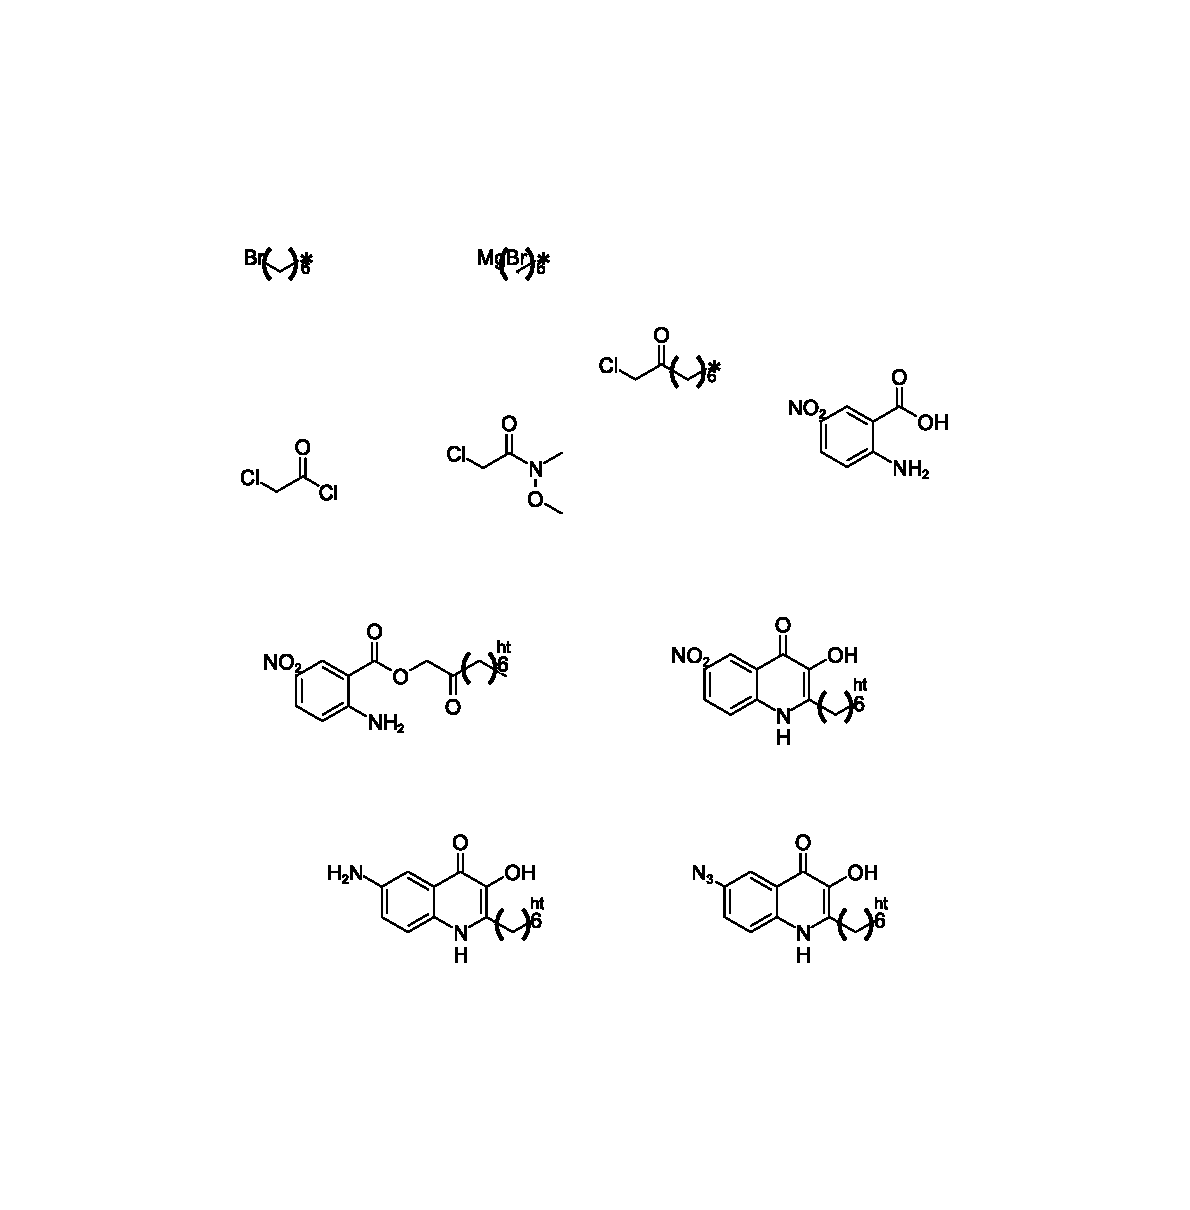
\includegraphics[width=\textwidth]{azPQS_synth}
		\caption{The synthesis of \compound{cmpd:azPQS}.
		a) Mg turnings, THF, r.t., 2 h then reflux, 2 h.
		b) \textit{N},\textit{O}-dimethylhydroxyl amine hydrochloride, \ce{K2CO3}, toluene, \ce{H2O}, - 5 $^{\circ}$C to r.t., 30 min, 71 \%.
		c) THF, 0 $^{\circ}$C to r.t., 15 h, 96 \%.
		d) \compound{cmpd:5naa}, \ce{K2CO3}, DMF, 90 $^{\circ}$C, 1 h, then \compound{cmpd:Clnon}, r.t., 18 h, 100 \%.
		e) Polyphosphoric acid, 90 $^{\circ}$C, 5.5 h, 40 \%.
		f) \ce{H2}, \ce{PtO2}, MeOH, 1 atm, r.t., 45 min, 80 \%.
		g) i) \ce{NaNO2}, HCl, \ce{H2O}, 0 $^{\circ}$C, 50 min. ii) \ce{NaN3}, \ce{H2O}, r.t., 4 h, 28 \% over two steps.
		\label{sch:azPQS_synth}}
	\end{center}
\end{scheme}

\subsection{C$_4$-HSL derivatives}

\subsubsection{Retrosynthesis of C$_4$-HSL derivatives \compound{cmpd:HL2N3}, \compound{cmpd:HL4N3} and \compound{cmpd:HL6N3}}

The azido analogue of C$_4$-HSL with a C$_2$ chain \compound{cmpd:HL2N3} (see \ref{fig:HL_anas}) has previously been prepared by Stacey \textit{et al.} \cite{Stacy2013}. It uses the cyclisation of \textsc{l}-methionine \compound{cmpd:LM} using bromoacetic acid via the mechanism shown in \ref{sch:HLHBr_mech} to form the homoserine lactone HBr salt \compound{cmpd:HLHBr}. This is then converted by a biphasic one-pot process to the azido-C$_2$ analogue \compound{cmpd:HL2N3} using bromoacetyl bromide \compound{cmpd:Br2Br} and \ce{NaN3}. It was hoped that this procedure could also be used to produce the azido-C$_4$ and C$_6$ chain analogues.

\begin{scheme}[H]
	\begin{center}
		\schemeref[LM]{cmpd:LM}
		\schemeref[HLHBr]{cmpd:HLHBr}
		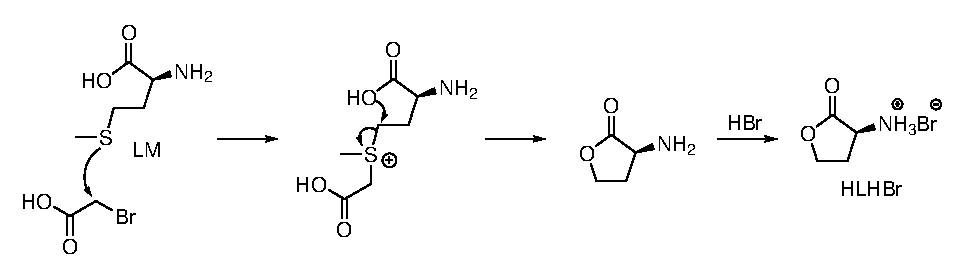
\includegraphics[width=\textwidth]{HLHBr_mech}
		\caption{The mechanism of formation of \compound{cmpd:HLHBr}. \label{sch:HLHBr_mech}}
	\end{center}
\end{scheme}

\begin{scheme}[H]
	\begin{center}
		\schemeref[LM]{cmpd:LM}
		\schemeref[HLHBr]{cmpd:HLHBr}
		\schemeref[Br2Br]{cmpd:Br2Br}
		\schemeref[Cl4Br]{cmpd:Cl4Br}
		\schemeref[Cl6Br]{cmpd:Cl6Br}
		\schemeref[HL2N3]{cmpd:HL2N3}
		\schemeref[HL4N3]{cmpd:HL4N3}
		\schemeref[HL6N3]{cmpd:HL6N3}
		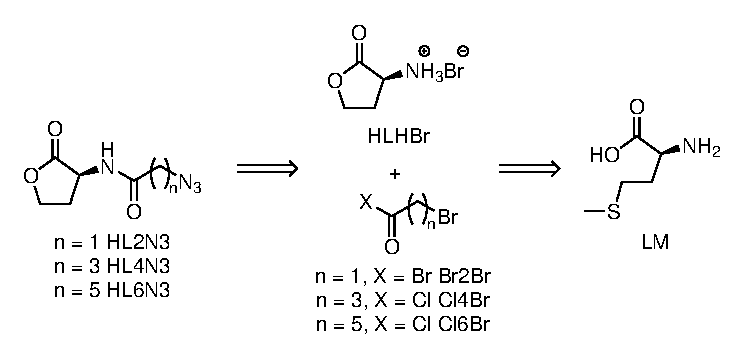
\includegraphics[width=\textwidth]{HL246N3_retro}
		\caption{The retrosynthesis of \compound{cmpd:HL2N3}, \compound{cmpd:HL4N3} and \compound{cmpd:HL6N3}. \label{sch:HL246N3_retro}}
	\end{center}
\end{scheme}

%\begin{scheme}[H]
%	\begin{center}
%		\schemeref[LM]{cmpd:LM}
%		\schemeref[HLHBr]{cmpd:HLHBr}
%		\schemeref[Br2Br]{cmpd:Br2Br}
%		\schemeref[HL2Br]{cmpd:HL2Br}
%		\schemeref[HL2N3]{cmpd:HL2N3}
%		\includegraphics[width=\textwidth]{HL2N3_retro}
%		\caption{The retrosynthesis of \compound{cmpd:HL2N3} \label{sch:HL2N3_retro}}
%	\end{center}
%\end{scheme}

\subsubsection{Synthesis of C$_4$-HSL derivatives \compound{cmpd:HL2N3}, \compound{cmpd:HL4N3} and \compound{cmpd:HL6N3}\label{sec:HL4N3}}

Homoserine lactone HBr salt \compound{cmpd:HLHBr} was synthesised using the procedure developed by Stacey \textit{et al.} \cite{Stacy2013}, followed by conversion to the azido-C$_2$ analogue \compound{cmpd:HL2N3} (see \ref{sch:HL2N3_synth}). Attempts to convert homoserine lactone \compound{cmpd:LM} to the azido-C$_4$ analogue using 4-bromobutyryl chloride \compound{cmpd:Cl4Br} produced a complex mixture of products. This is likely to be because the S$_N$2 reaction where the azide anion displaces bromine is slower as the bromine atom being displaced is no longer next to a carbonyl group. Hence, this allows more side reactions to occur instead of the desired reaction. It was therefore decided that the conversion should be carried out as a two-step process, where a bromoacyl chain is first installed, followed by the S$_N$2 reaction with \ce{NaN3} (see \ref{sch:HL46N3_synth}). 

Reaction of the homoserine lactone HBr salt \compound{cmpd:HLHBr} with 4-bromobutyryl chloride \compound{cmpd:Cl4Br} or 6-bromohexanoyl chloride \compound{cmpd:Cl6Br} produced bromo-C$_4$ analogue \compound{cmpd:HL4Br} or bromo-C$_6$ analogue \compound{cmpd:HL6Br} respectively. Heating with \ce{NaN3} in DMF converted bromo-C$_6$ analogue \compound{cmpd:HL6Br} to azido-C$_6$ analogue \compound{cmpd:HL6N3}\cite{Baker2012}. It is hoped that the same conditions can be used to convert bromo-C$_4$ analogue \compound{cmpd:HL4Br} to azido-C$_4$ analogue \compound{cmpd:HL4N3} and this will be attempted shortly.

\begin{scheme}[H]
	\begin{center}
		\schemeref[LM]{cmpd:LM}
		\schemeref[HLHBr]{cmpd:HLHBr}
		\schemeref[Br2Br]{cmpd:Br2Br}
		\schemeref[HL2N3]{cmpd:HL2N3}
		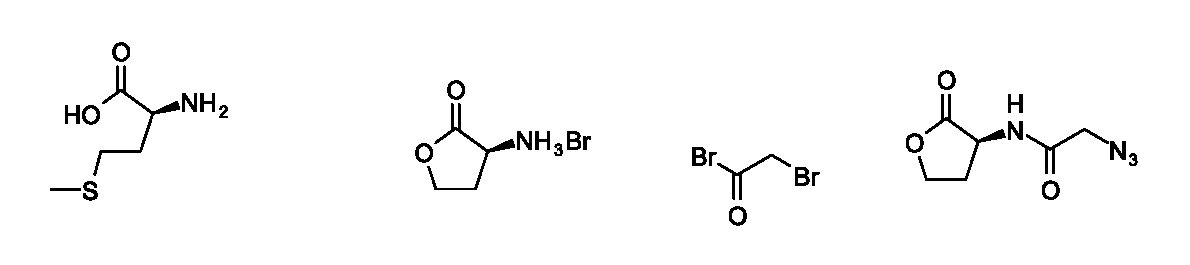
\includegraphics[width=\textwidth]{HL2N3_synth}
		\caption{The synthesis of \compound{cmpd:HL2N3}.
		a) Bromoacetic acid, \textit{i}-PrOH:\ce{H2O}:AcOH (5:5:2), r.t., 18 h, 41 \%.
		b) \ce{NaN3}, \ce{NaHCO3}, \ce{H2O}/\ce{CH2Cl2}, r.t., 18 h, 41 \%.
		\label{sch:HL2N3_synth}}
	\end{center}
\end{scheme}
%
%\begin{scheme}[H]
%	\begin{center}
%		\schemeref[LM]{cmpd:LM}
%		\schemeref[HLHBr]{cmpd:HLHBr}
%		\schemeref[Cl4Br]{cmpd:Cl4Br}
%		\schemeref[Cl6Br]{cmpd:Cl6Br}
%		\schemeref[HL4Br]{cmpd:HL4Br}
%		\schemeref[HL6Br]{cmpd:HL6Br}
%		\schemeref[HL4N3]{cmpd:HL4N3}
%		\schemeref[HL6N3]{cmpd:HL6N3}
%		\includegraphics[width=\textwidth]{HL46N3_retro}
%		\caption{The retrosynthesis of \compound{cmpd:HL4N3} and \compound{cmpd:HL6N3} \label{sch:HL46N3_retro}}
%	\end{center}
%\end{scheme}

\begin{scheme}[H]
	\begin{center}
		\schemeref[LM]{cmpd:LM}
		\schemeref[HLHBr]{cmpd:HLHBr}
		\schemeref[Cl4Br]{cmpd:Cl4Br}
		\schemeref[Cl6Br]{cmpd:Cl6Br}
		\schemeref[HL4Br]{cmpd:HL4Br}
		\schemeref[HL6Br]{cmpd:HL6Br}
		\schemeref[HL4N3]{cmpd:HL4N3}
		\schemeref[HL6N3]{cmpd:HL6N3}
		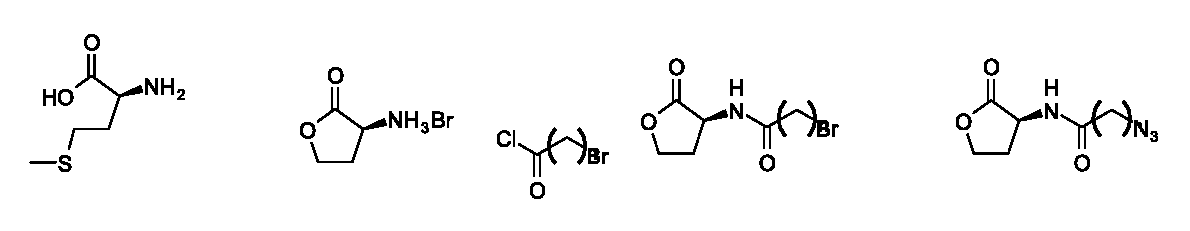
\includegraphics[width=\textwidth]{HL46N3_synth}
		\caption{The synthesis of \compound{cmpd:HL4N3} and \compound{cmpd:HL6N3}.
		a) Bromoacetic acid, \textit{i}-PrOH:\ce{H2O}:AcOH (5:5:2), r.t, 18 h, 41 \%.
		b) \ce{NaHCO3}, \ce{H2O}/\ce{CH2Cl2}, r.t., 18 h, \compound{cmpd:HL4Br} : 80 \%, \compound{cmpd:HL6Br} : 66 \%.
		c) \ce{NaN3}, DMF, 100 $^{\circ}$C, 5 h, \compound{cmpd:HL6N3} : 56 \%.
		\label{sch:HL46N3_synth}}
	\end{center}
\end{scheme}

\subsection{3-oxo-C$_{12}$-HSL derivative \compound{cmpd:HLO12N3}}

\subsubsection{Synthesis of 3-oxo-C$_{12}$-HSL derivative \compound{cmpd:HLO12N3}}

The aim of this project is to contribute a new component to this library by synthesising an azido analogue of 3-oxo-C$_{12}$-HSL \compound{cmpd:HLO12} (see \ref{fgr:PA_QSMs}). The synthesis of this analogue, 3-oxo-12-azido-C$_{12}$-HSL \compound{cmpd:HLO12N3}, is shown in \ref{sch:HLO12N3_synth}\cite{Hodgkinson2011b, Amara2009,Garner2011}. This synthesis follows a route devised in the Spring group for the synthesis of 3-oxo-C$_{12}$-HSL \compound{cmpd:HLO12}\cite{Hodgkinson2011b}, but uses 10-azidodecanoyl chloride \compound{cmpd:Cl10N3} rather than decanoyl chloride. Analogues with shorter or longer tail lengths (known to affect selectivity and binding affinity) could also be synthesised using the same method. 

%\begin{scheme}[H]
%	\begin{center}
%		\schemeref[HLO12N3]{cmpd:HLO12N3}
%		\schemeref[Y4PipFOxaAmAc]{cmpd:Y4PipFOxaAmAc}
%		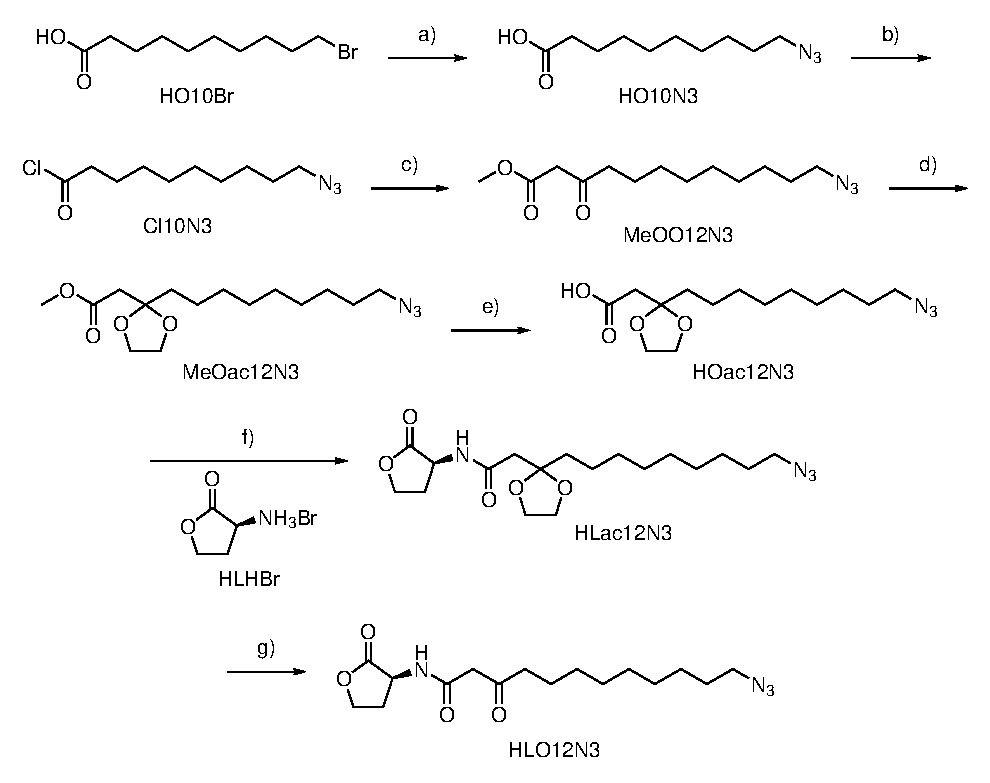
\includegraphics[width=\textwidth]{HLO12N3_synth}
%		\caption{Proposed synthesis of 3-oxo-C$_12$-HSL analogue \compound{cmpd:HLO12N3}.}
%		\label{sch:HLO12N3_synth}}
%	\end{center}
%\end{scheme}

\begin{scheme}[H]
	\begin{center}
		\schemeref[HO10Br]{cmpd:HO10Br}
		\schemeref[HO10N3]{cmpd:HO10N3}
		\schemeref[Cl10N3]{cmpd:Cl10N3}
		\schemeref[Mel]{cmpd:Mel}
		\schemeref[Mel10N3]{cmpd:Mel10N3}
		\schemeref[MeOO12N3]{cmpd:MeOO12N3}
		\schemeref[MeOac12N3]{cmpd:MeOac12N3}
		\schemeref[HOac12N3]{cmpd:HOac12N3}
		\schemeref[HLHBr]{cmpd:HLHBr}
		\schemeref[HLac12N3]{cmpd:HLac12N3}
		\schemeref[HLO12N3]{cmpd:HLO12N3}
		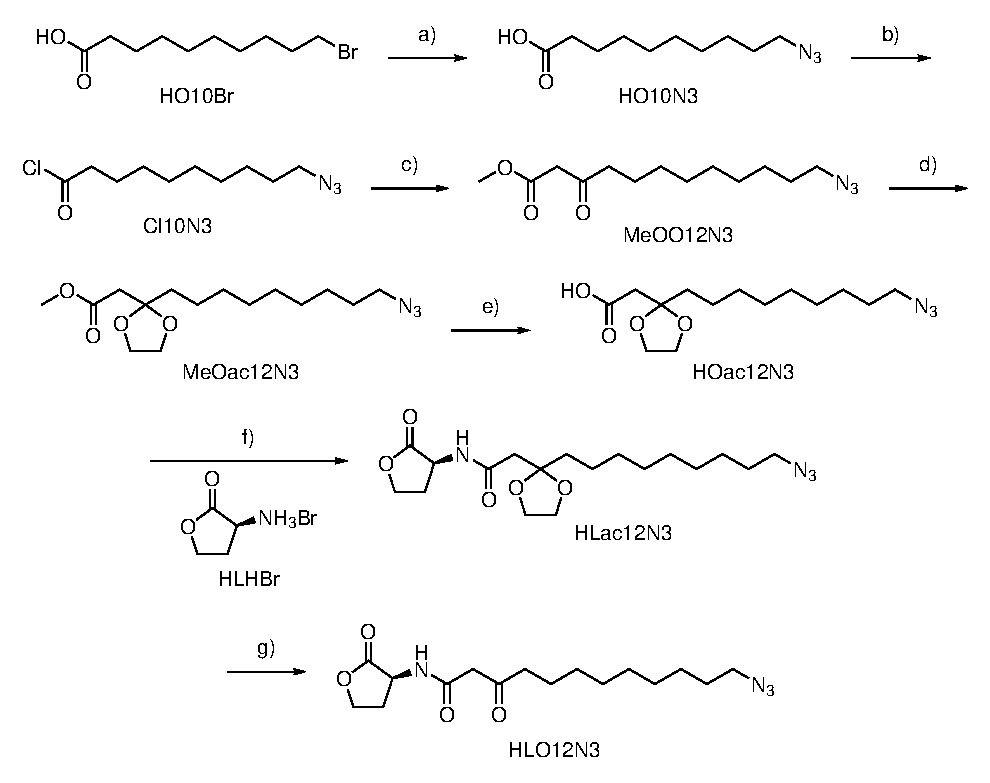
\includegraphics[width=\textwidth]{HLO12N3_synth}
		\caption{Proposed synthesis of 3-oxo-C$_{12}$-HSL analogue \compound{cmpd:HLO12N3}.
		a) \ce{NaN3}, DMF, $50\ ^{\circ}$C\cite{Khoukhi1987}.
		b) Oxalyl chloride, DMF, \ce{CH2Cl2}, rt\cite{Chaturvedi2012,Khoukhi1987}.
		c) pyridine, DCM, $0\ ^{\circ}$C\cite{Khoukhi1987, Hodgkinson2011b}. 
		d) MeOH, reflux\cite{Khoukhi1987, Hodgkinson2011b}.
		e) \textit{p}-TsOH, \ce{HO(CH2)2OH}, \ce{CH(OMe)3}, rt\cite{Hodgkinson2011b}.
		f) NaOH, \ce{H2O}, rt\cite{Hodgkinson2011b}.
		g) EDC, DMAP, \ce{CH2Cl2}, rt\cite{Hodgkinson2011b}.
		h) TFA, rt\cite{Hodgkinson2011b}. 
		\label{sch:HLO12N3_synth}}
	\end{center}
\end{scheme}

\newpage

\section{Antibiotic analogues}

\subsection{Ciprofloxacin derivatives}

Ciprofloxacin \compound{cmpd:cip} (see \ref{fgr:cip_num}) is second-generation fluoroquinolone antibiotic used to treat both Gram-positive and Gram-negative bacterial infections\cite{Oliphant2002}.
The structure-activity relationships for ciprofloxacin have been investigated \cite{Renau1996} and positions 2 and 7 were found not to cause loss of activity. It was therefore decided that alkyne tails would be added at these positions giving two analogues of ciprofloxacin, \compound{cmpd:hexpipcip} and \compound{cmpd:pipciphex} (see \ref{sch:cip_anas}).

Three derivatives of ciprofloxacin modified at the free piperazine N were synthesised. These contained a six-carbon alkyl chain with a terminal alkyne, a six-carbon acyl chain with a terminal alkyne and a three carbon acyl chain with a terminal alkyne.

\subsubsection{Retrosynthesis of ciprofloxacin analogue \compound{cmpd:hexpipcip}}

The retrosynthesis of ciprofloxacin analogue \compound{cmpd:hexpipcip} is shown in \ref{sch:hexpipcip_retro}.
The analogue has has an alkyne tail attached on the free piperazine N; it is more convenient to attach the alkyne chain to piperazine before coupling of the alkyl piperazine \compound{cmpd:hexpip} to the ciprofloxacin core \compound{cmpd:Clcip} as this method is more convergent. This can be achieved by reductive amination of hex-5-ynal \compound{cmpd:hexynal} with 1-boc-piperazine \compound{cmpd:pipboc} followed by deprotection to form the alkyl piperazine \compound{cmpd:hexpip}. This method was found by Renau \textit{et al.} to be "...superior to previous reports which involved alkylation of piperazine with an appropriate alkyl halide." \cite{Renau1996,JPS:JPS2600571210}. 
S$_N$Ar coupling of the piperazine derivative with ciprofloxacin precursor \compound{cmpd:Clcip} leads to the final analogue \compound{cmpd:hexpipcip}.

\begin{scheme}[H]
	\begin{center}
		\schemeref[hexynol]{cmpd:hexynol}
		\schemeref[hexynal]{cmpd:hexynal}
		\schemeref[pipboc]{cmpd:pipboc}
		\schemeref[hexpipboc]{cmpd:hexpipboc}
		\schemeref[hexpip]{cmpd:hexpip}
		\schemeref[Clcip]{cmpd:Clcip}
		\schemeref[hexpipcip]{cmpd:hexpipcip}
		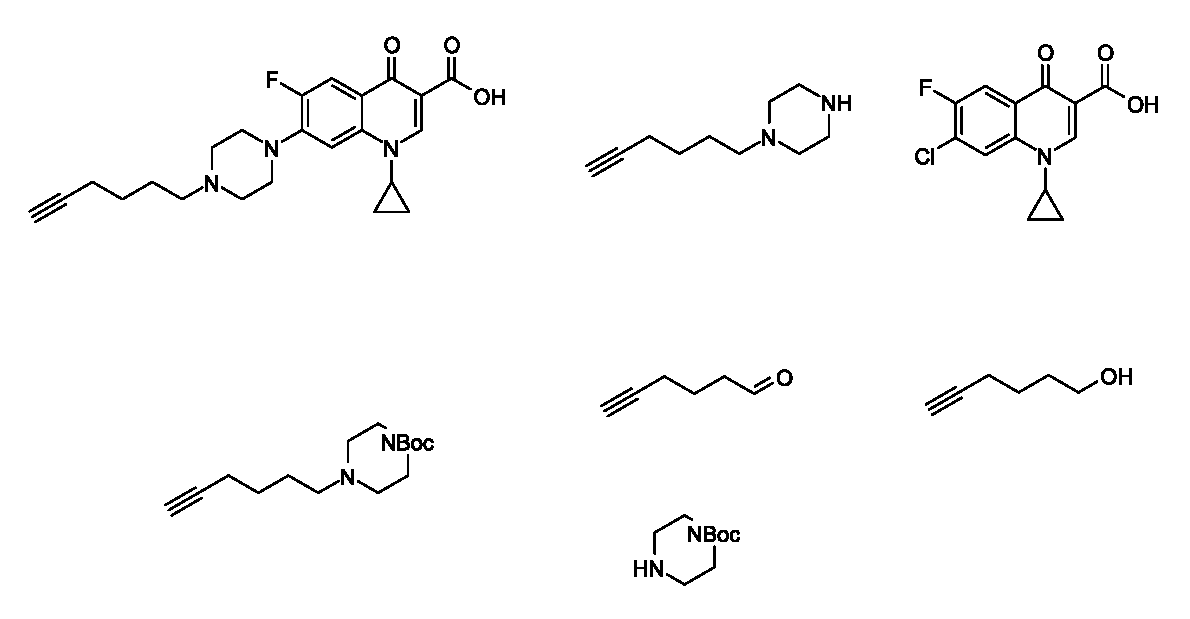
\includegraphics[width=\textwidth]{hexpipcip_retro}
		\caption{The retrosynthesis of \compound{cmpd:hexpipcip}. \label{sch:hexpipcip_retro}}
	\end{center}
\end{scheme}

\subsubsection{Synthesis of ciprofloxacin analogue \compound{cmpd:hexpipcip}}

The synthesis of \compound{cmpd:hexpipcip} follows the strategy followed by Renau \textit{et al.} \cite{Renau1996}. Unlike the aldehydes and ketones used by Renau \textit{et al.}\cite{Renau1996}, hex-5-ynal \compound{cmpd:hexynal} is not commercially available and so was successfully prepared by PCC oxidation of hex-5-ynol \compound{cmpd:hexynol} according to the procedure described by Kocsis \textit{et al.} \cite{Kocsis2012}. Renau \textit{et al.}\cite{Renau1996} used sodium cyanoborohydride to facilitate the reductive amination of hex-5-ynal \compound{cmpd:hexynal} and 1-Boc-piperazine \compound{cmpd:pipboc}. However, it was decided to attempt this transformation using the less toxic sodium triacetoxyborohydride following a procedure reported by Abdel-Magid \textit{et al.} \cite{Abdel-Magid1996}. This reaction yielded compound \compound{cmpd:hexpipboc}, which was deprotected using TFA using the procedure described by Renau \textit{et al.}\cite{Renau1996} to give compound \compound{cmpd:hexpip}. This was refluxed in MeCN with the commercially available ciprofloxacin precursor \compound{cmpd:Clcip} according to the procedure described by Renau \textit{et al.}\cite{Renau1996}, however the reaction did not proceed. Addition of \ce{NEt3} did not lead to reaction, however it was found that refluxing in neat \ce{NEt3} lead to conversion to the final ciprofloxacin analogue \compound{cmpd:hexpipcip}.

\begin{scheme}[H]
	\begin{center}
		\schemeref[hexynol]{cmpd:hexynol}
		\schemeref[hexynal]{cmpd:hexynal}
		\schemeref[pipboc]{cmpd:pipboc}
		\schemeref[hexpipboc]{cmpd:hexpipboc}
		\schemeref[hexpip]{cmpd:hexpip}
		\schemeref[Clcip]{cmpd:Clcip}
		\schemeref[hexpipcip]{cmpd:hexpipcip}
		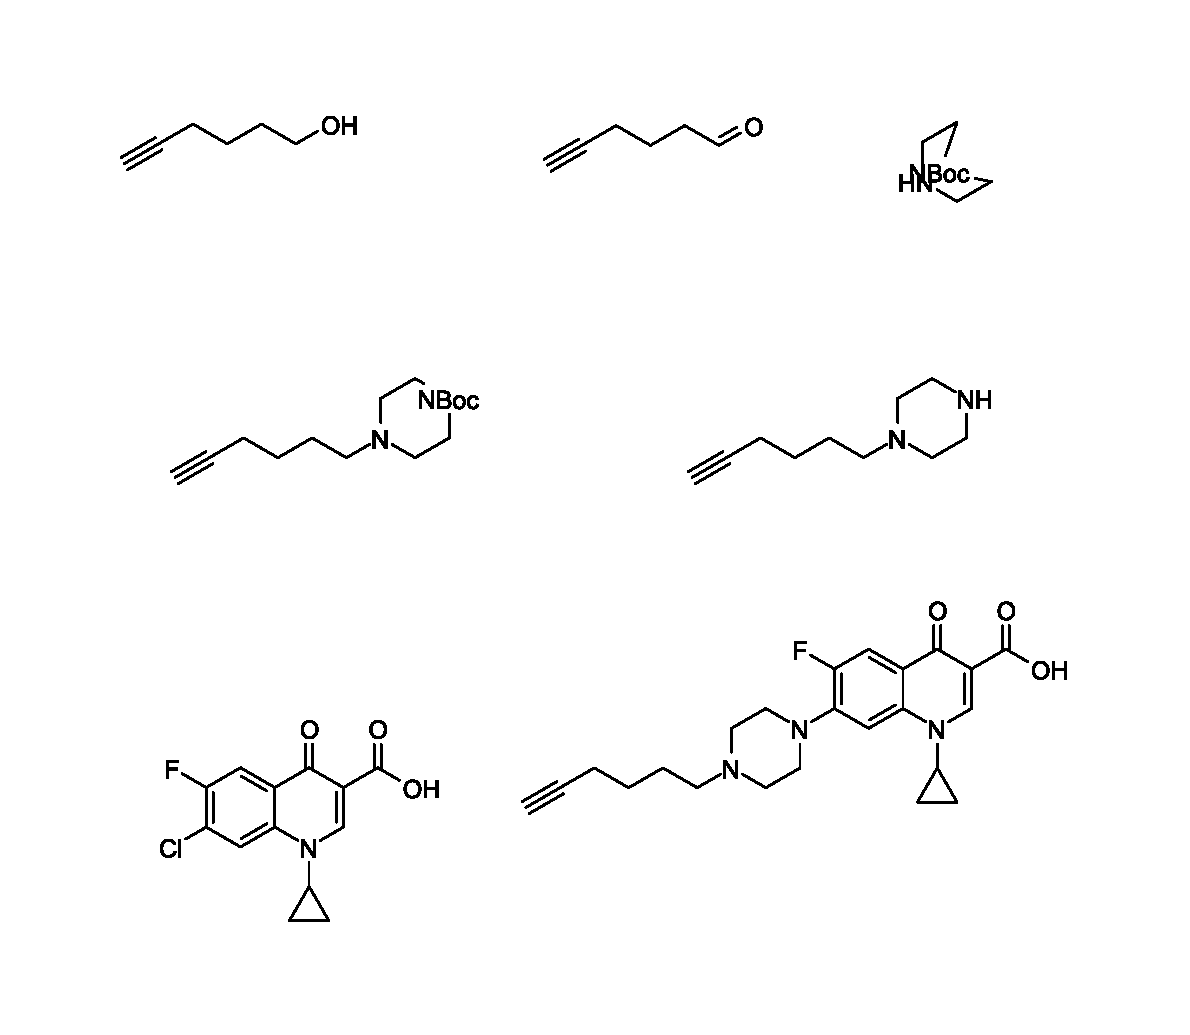
\includegraphics[width=\textwidth]{hexpipcip_synth}
		\caption{The synthesis of \compound{cmpd:hexpipcip}. 
		a) Pyridinium chlorochromate, \ce{CH2Cl2}, r.t., 5 h, 72 \%.
		b) \ce{NaBH(AcO)3}, 1,2-dichloroethane, r.t., 10.5 h, 99 \%.
		c) TFA, r.t., 1 h, 100 \%.
		d) \ce{NEt3}, reflux, 15 h, 21 \%. %weigh
		\label{sch:hexpipcip_synth}}
	\end{center}
\end{scheme}

\subsection{Trimethoprim derivatives}

\begin{scheme}[H]
	\begin{center}
		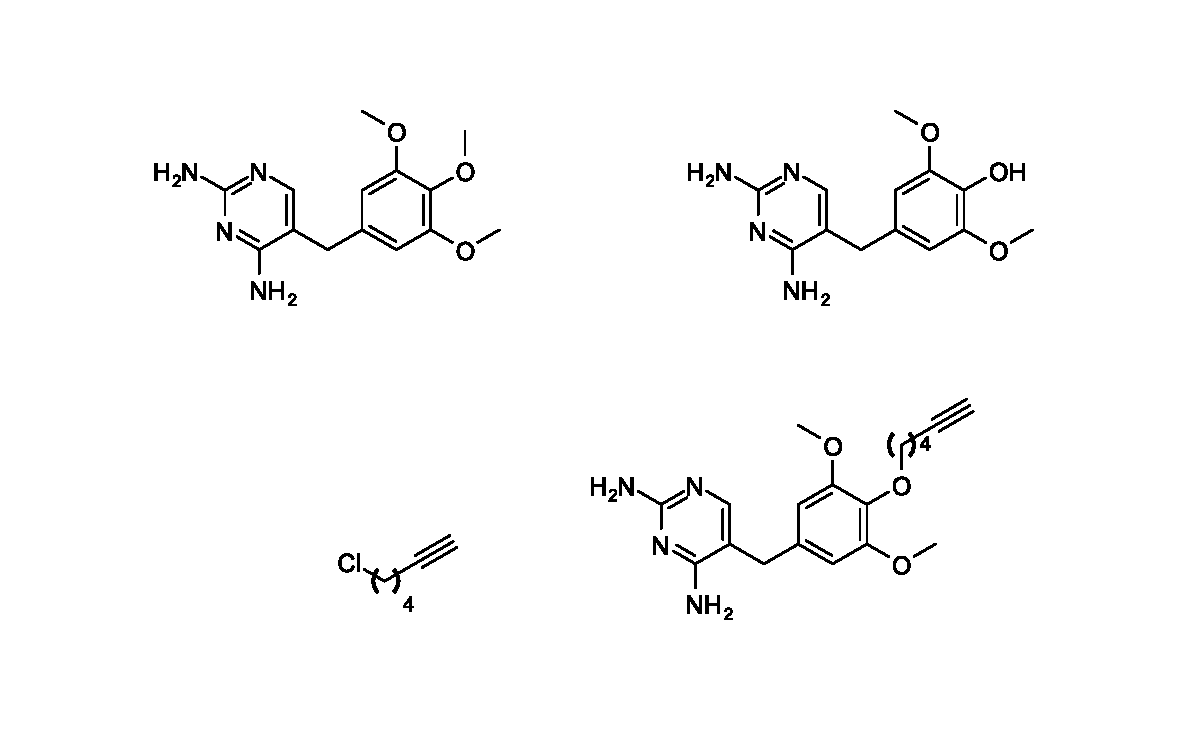
\includegraphics[width=\textwidth]{Y4Tri_synth}
		\caption{\label{sch:}}
	\end{center}
\end{scheme}

\subsection{Sulfanilamide derivative}

Sulfanilamide antibiotics were the first class to be widely used\cite{Otten1986,Wainwright2011}. The first drug in the class was called Prontosil \compound{cmpd:Pron} and was developed by Bayer and first patented in 1937. Prontosil \compound{cmpd:Pron} is inactive in vitro but active in vivo, as it is a prodrug which is reduced in vivo to release the active drug, sulfanilamide \compound{cmpd:Sul}, and 1,2,4-triaminobenzene \compound{cmpd:124am} (see \ref{fig:Pron}).



\begin{scheme}[H]
	\begin{center}
	\schemeref[Pron]{cmpd:Pron}
	\schemeref[Sul]{cmpd:Sul}
	\schemeref[124am]{cmpd:124am}
		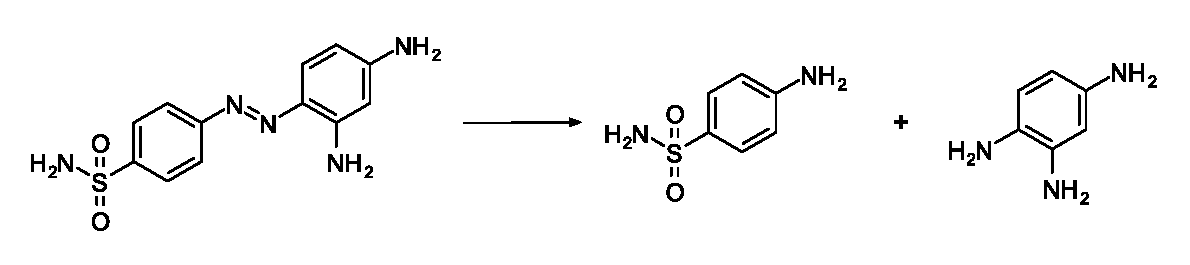
\includegraphics[width=\textwidth]{Pron}
		\caption{The reduction of Prontosil \compound{cmpd:Pron} to release sulfanilamide \compound{cmpd:Sul} and 1,2,4-triaminobenzene \compound{cmpd:124am}.
		\label{fig:Pron}}
	\end{center}
\end{scheme}

Analogues of sulfaniliamide \compound{cmpd:Sul} have previously been synthesised using a click reaction to append different R groups\cite{Wang2010} (see \ref{sch:Y1Sul_click}). However, if one considers sulfonamide antibiotics already in use, all except sulfacetamide have a heterocycle linked directly to the sulfur atom, rather than with a methylene group in between (see \ref{fig:Sul_ABs}). 

\begin{scheme}[H]
	\begin{center}
		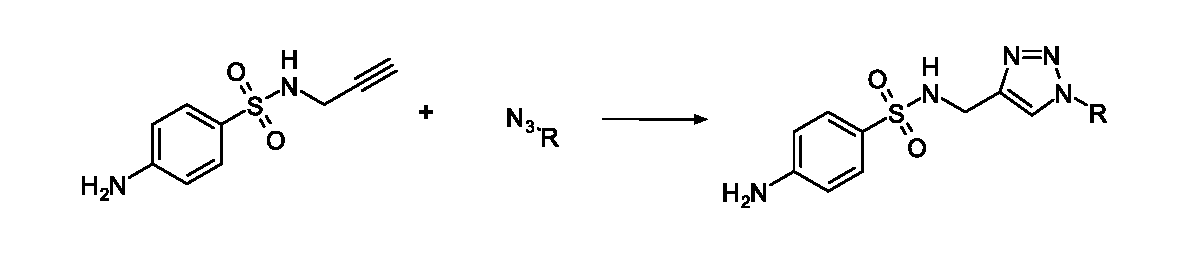
\includegraphics[width=\textwidth]{Y1Sul_click}
		\caption{The sulfanilamide analogues synthesised using click chemistry by Wang et al\cite{Wang2010}.
		\label{sch:Y1Sul_click}}
	\end{center}
\end{scheme}

\begin{scheme}[H]
	\begin{center}
		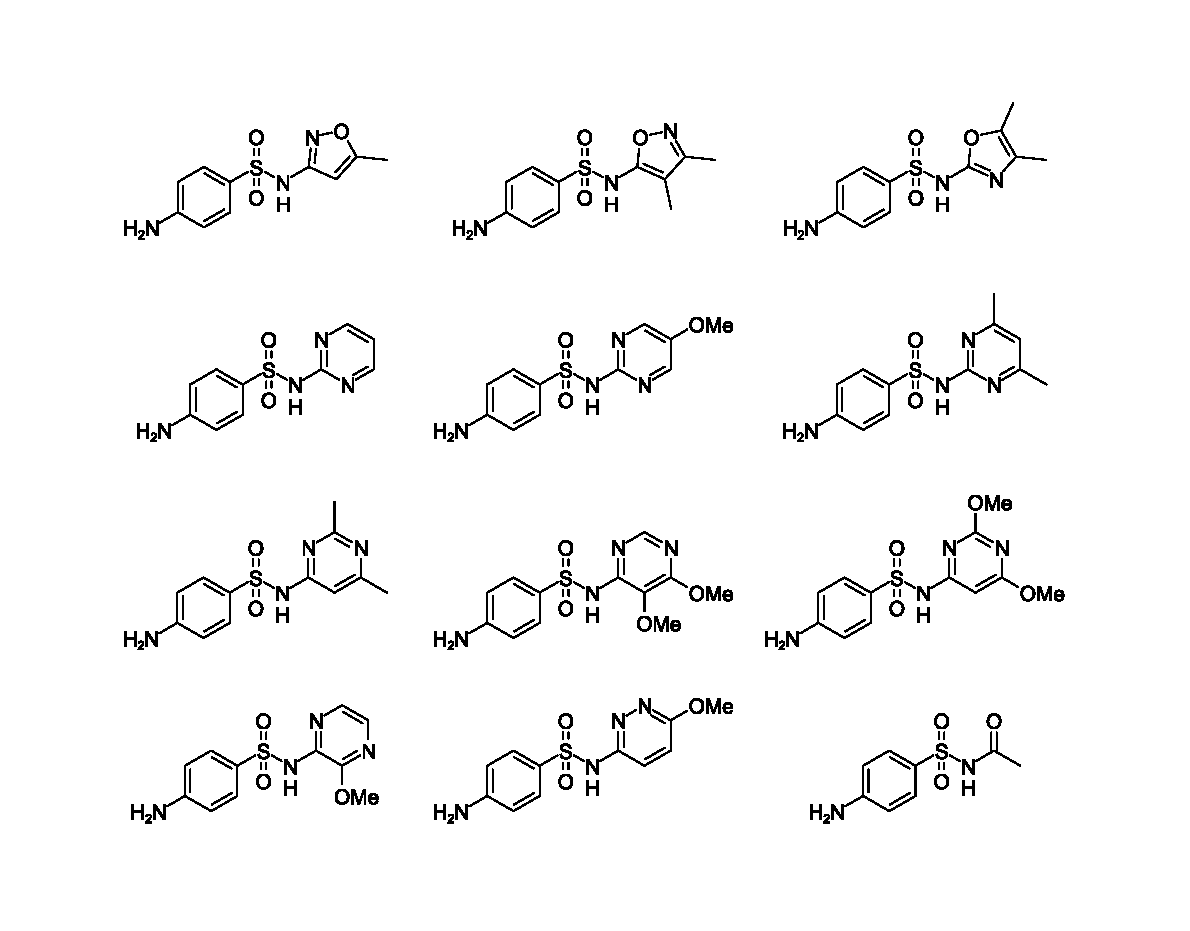
\includegraphics[width=\textwidth]{Sul_ABs}
		\caption{Sulfonamide antibiotics.
		\label{fig:Sul_ABs}}
	\end{center}
\end{scheme}

Therefore, it is postulated that a 1,2,3-triazole could be introduced in the position occupied by a heterocycle in other known sulfonamide antibiotics by attachment of an alkyne directly to the sulfonamide nitrogen to form compound \compound{cmpd:Y0Sul} or a protected version of it (see \ref{sch:Y0Sul_idea}).

\begin{scheme}[H]
	\begin{center}
	\schemeref[Y0Sul]{cmpd:Y0Sul}
		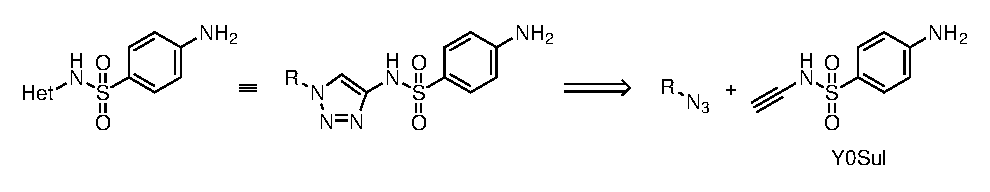
\includegraphics[width=\textwidth]{Y0Sul_idea}
		\caption{Retrosynthesis of a 1,2,3-triazole-containing sulfonamide antibiotic-autoinducer hybrid.
		\label{sch:Y0Sul_idea}}
	\end{center}
\end{scheme}

\subsubsection{Retrosynthesis of sulfanilimide analogue \compound{cmpd:Y0Sul}}

It is hoped that sulfanilamide analogue \compound{cmpd:Y0Sul} could be synthesised and reacted with the azido autoinducer analogues directly. This would allow a more efficient synthesis of the library, as no deprotection steps would be needed after the click reaction. However, it appears that no secondary ynamides have been synthesised to date\cite{ScifinderSecondaryYnamide}.
Documents referring to the synthesis of secondary ynamides are either missing \cite{Vellanki2013}, do not refer to the reaction catalogued by Scifinder\cite{Yamaguchi2013,Kaiser2010,Zavyalov1967}, refer compounds containing proparagyl groups instead of ynamides\cite{Gnaccarini2012,Wang2012,Rajopadhye2007,LeitDeMoradeiMarcela2006} or mention unlikely reactions with ethynamine\cite{Edmondson2013} or a derivative\cite{Fujimaki1999} without mentioning how these precursors were synthesised. Scifinder does not have a synthesis of ethynamine, suggesting that it is too unstable to form, but does have two papers discussing the syntheses of other primary ynamines \cite{Shvartsberg1976,Hill1998}.

\begin{scheme}[H]
	\begin{center}
		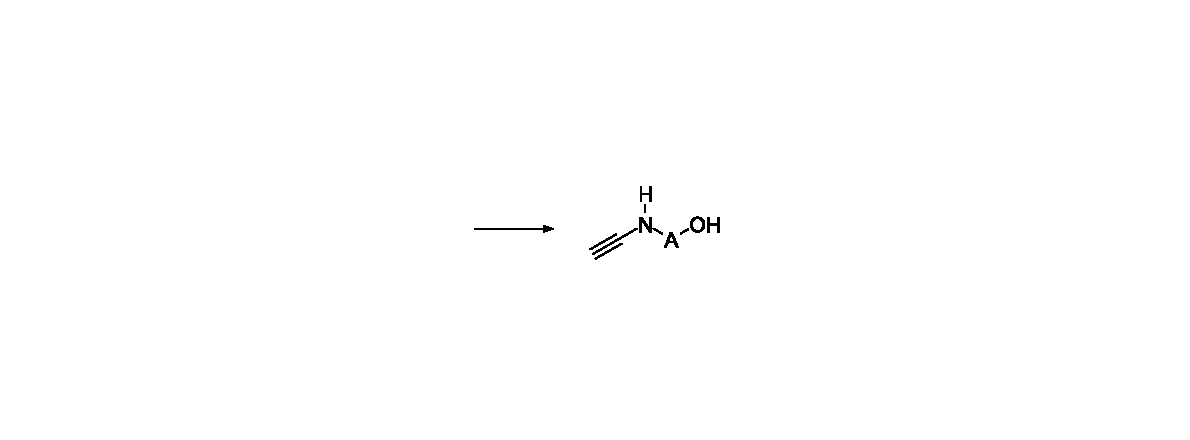
\includegraphics[width=\textwidth]{Scifinder}
		\caption{The Scifinder reaction substructure search used to show that secondary ynamides have not yet been synthesised\cite{ScifinderSecondaryYnamide}.
		\label{fig:Scifinder}}
	\end{center}
\end{scheme}

\begin{scheme}[H]
	\begin{center}
		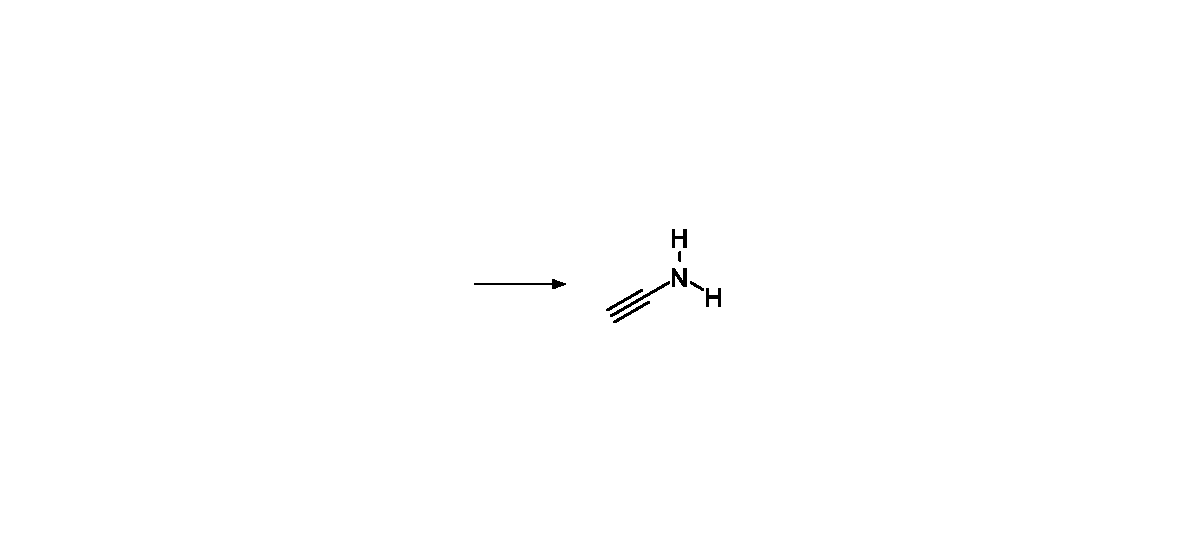
\includegraphics[width=\textwidth]{Scifinder_primary_ynamine}
		\caption{The Scifinder reaction substructure search used to find the synthses of primary ynamines\cite{ScifinderPrimaryYnamine}.
		\label{fig:Scifinder_primary_ynamine}}
	\end{center}
\end{scheme}


Conversely, the synthesis of tertiary ynamines has been studied more widely\cite{Ficini1976}. In particular, tertiary ynamides (often defined as ynamines with any electron-withdrawing group attached) have been shown to be relatively stable and easy to work with in reactions including 
addition at the $\alpha$ position, 
addition at the $\beta$ position, 
reduction/reductive coupling
oxidation,
cycloaddition, 
ring-closing metathesis,
cycloisomerisation,
functionalisation of terminal ynamides and click reactions\cite{IJsselstijn2006,Evano2010}. 

The study of click reactions of ynamides by IJsselstijn et al. uses terminal ynamides protected using a benzyl and a tosyl group or a benzyl and a benzoyl group. Although their click reactions proceed with high yield, they fail to present the deprotection of their final compounds. However, these reactions provide a promising suggestion that click reactions between a protected sulfanilamide derivative and the azido-autoinducer derivatives are feasible. The tosyl group used by IJsselstijn et al. to protect their ynamide is very similar to the \textit{p}-aminobenzenesulfonyl group needed in the alkynyl-sulfanilamide derivative. However, installation of the alkyne could be problematic in the presence of a second amine, so the \ce{NH2} group is installed as a \ce{NO2} group and reduced after the click reaction.  Similarly, the benzyl protecting group must be removed after the click reaction.

\begin{scheme}[H]
	\begin{center}
	\schemeref[PMBa]{cmpd:PMBa}
	\schemeref[NsCl]{cmpd:NsCl}
	\schemeref[TIPSY]{cmpd:TIPSY}
	\schemeref[TIPSYBr]{cmpd:TIPSYBr}
	\schemeref[NsPMB]{cmpd:NsPMB}
	\schemeref[TIPSYNsPMB]{cmpd:TIPSYNsPMB}
	\schemeref[YNsPMB]{cmpd:YNsPMB}
	\schemeref[HL2N3]{cmpd:HL2N3}
	\schemeref[HL2TNsPMB]{cmpd:HL2TNsPMB}
	\schemeref[HL2T0Sul]{cmpd:HL2T0Sul}
		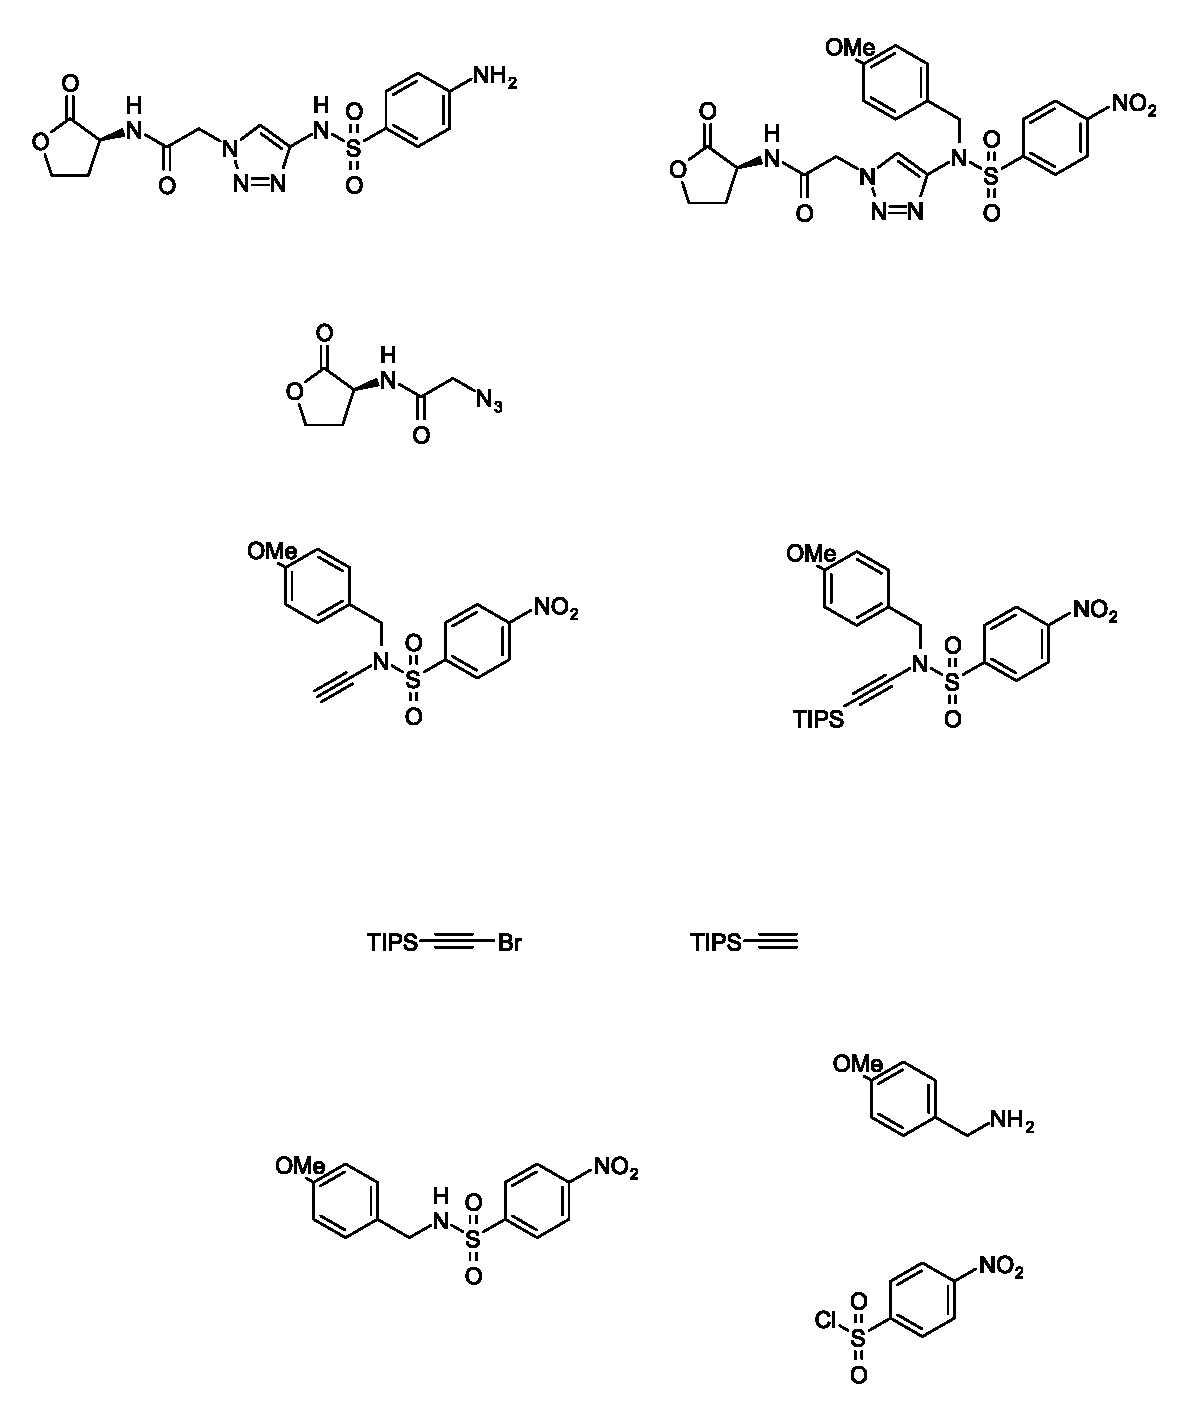
\includegraphics[width=\textwidth]{HL2T0Sul_retro}
		\caption{Retrosynthesis of a 1,2,3-triazole-containing sulfonamide antibiotic-autoinducer hybrid.
		\label{sch:HL2T0Sul_retro}}
	\end{center}
\end{scheme}

\subsubsection{Synthesis of sulfanilimide analogue \compound{cmpd:Y0Sul}}

\begin{scheme}[H]
	\begin{center}
	\schemeref[PMBa]{cmpd:PMBa}
	\schemeref[NsCl]{cmpd:NsCl}
	\schemeref[TIPSY]{cmpd:TIPSY}
	\schemeref[TIPSYBr]{cmpd:TIPSYBr}
	\schemeref[NsPMB]{cmpd:NsPMB}
	\schemeref[TIPSYNsPMB]{cmpd:TIPSYNsPMB}
	\schemeref[YNsPMB]{cmpd:YNsPMB}
	\schemeref[HL2N3]{cmpd:HL2N3}
	\schemeref[HL2TNsPMB]{cmpd:HL2TNsPMB}
	\schemeref[HL2T0Sul]{cmpd:HL2T0Sul}
		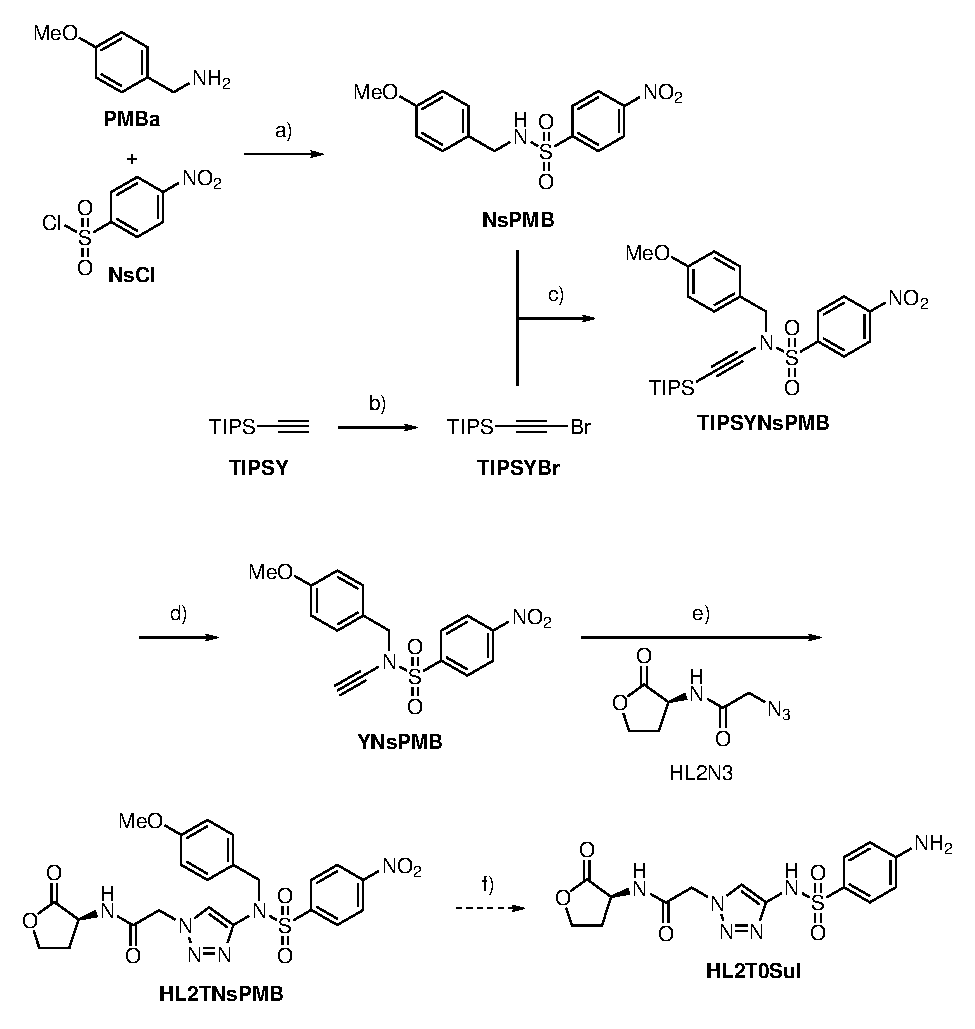
\includegraphics[width=\textwidth]{HL2T0Sul_synth}
		\caption{Synthesis of a 1,2,3-triazole-containing sulfonamide antibiotic-autoinducer hybrid.
		a) \ce{CH2Cl2}, r.t., 24 h \cite{Bendikov2005}. 
		b) \ce{AgNO3}, acetone, r.t., 3 h \cite{Graux2014}. 
		c) \ce{CuSO4.5H2O}, 1,10-phenanthroline, \ce{K2CO3}, toluene, $80\ ^{\circ}$C, 48 h \cite{Graux2014}. 
		d) TBAF, THF, $-78\ ^{\circ}$C, 3 h\cite{Graux2014}. 
		e) \ce{Cu(OAc)2}, sodium ascorbate, \ce{CH2Cl2}, \textit{t}-BuOH, \ce{H2O}, r.t., 16 h \cite{IJsselstijn2006}. 
		f) \ce{SnCl2}, TFA, \ce{CH2Cl2}, reflux, 3 h \cite{Bissinger2011, Reuillon2012}.
		\label{sch:HL2T0Sul_synth}}
	\end{center}
\end{scheme}

%\subsubsection{Retrosynthesis of sulfanilimide analogues \compound{cmpd:Y1Sul} and \compound{cmpd:Y4Sul}}

\subsection{Linezolid derivative}

\subsubsection{Retrosynthesis of linezolid analogue \compound{cmpd:Y0Lin}}

If time permits, an alkynyl analogue of the antibiotic linezolid \compound{cmpd:Lin} (see \ref{fgr:ABs}) could also be synthesised. The route follows a recent literature procedure described by Phetsang \textit{et al}.\cite{Phetsang2014}. The morpholine ring of linezolid is replaced by piperazine, allowing an alkynyl tail to be attached to the molecule (as opposed to the azido tail attached by Phetsang \textit{et al}.).

\begin{scheme}[H]
	\begin{center}
		\schemeref[2FN]{cmpd:2FN}
		\schemeref[Pip]{cmpd:Pip}
		\schemeref[PipFN]{cmpd:PipFN}
		\schemeref[PipFAm]{cmpd:PipFAm}
		\schemeref[CbzPipFAmCbz]{cmpd:CbzPipFAmCbz}
		\schemeref[RGlyBu]{cmpd:RGlyBu}
		\schemeref[CbzPipFOxaOH]{cmpd:CbzPipFOxaOH}
		\schemeref[CbzPipFOxaOTs]{cmpd:CbzPipFOxaOTs}
		\schemeref[KPhth]{cmpd:KPhth}
		\schemeref[CbzPipFOxaPhth]{cmpd:CbzPipFOxaPhth}
		\schemeref[CbzPipFOxaAm]{cmpd:CbzPipFOxaAm}
		\schemeref[CbzPipFOxaAmAc]{cmpd:CbzPipFOxaAmAc}
		\schemeref[PipFOxaAmAc]{cmpd:PipFOxaAmAc}
		\schemeref[Y4I]{cmpd:Y4I}
		\schemeref[Y4PipFOxaAmAc]{cmpd:Y4PipFOxaAmAc}
		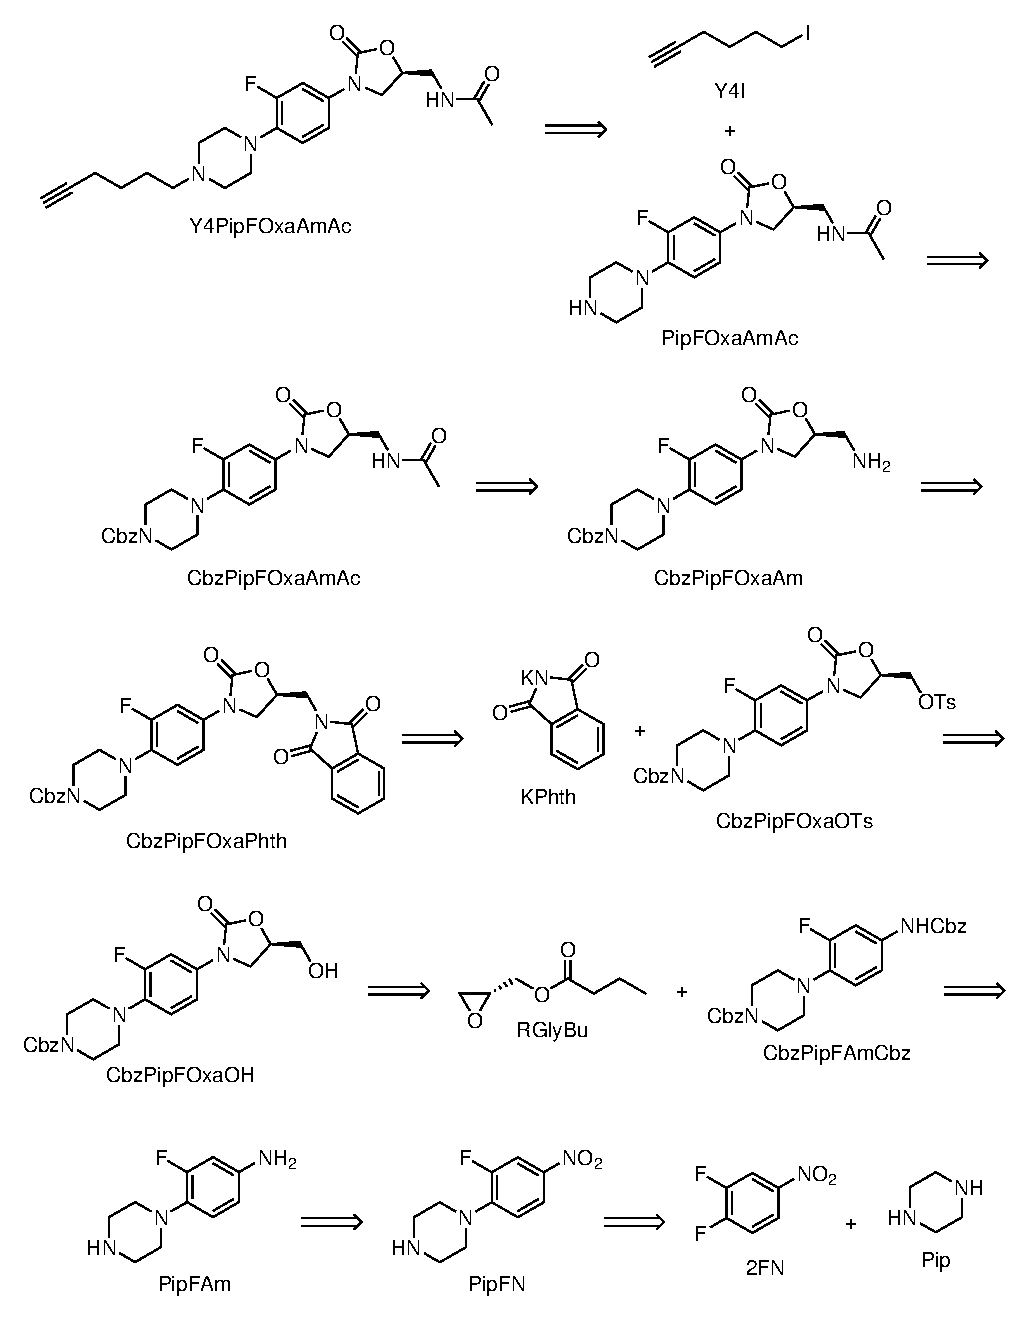
\includegraphics[width=\textwidth]{YLin_retro}
		\caption{Retrosynthesis of linezolid analogue \compound{cmpd:YLin}\cite{Phetsang2014}.
		\label{sch:YLin_retro}}
	\end{center}
\end{scheme}

\subsubsection{Synthesis of linezolid analogue \compound{cmpd:Y0Lin}}

\begin{scheme}[H]
	\begin{center}
		\schemeref[2FN]{cmpd:2FN}
		\schemeref[Pip]{cmpd:Pip}
		\schemeref[PipFN]{cmpd:PipFN}
		\schemeref[PipFAm]{cmpd:PipFAm}
		\schemeref[CbzPipFAmCbz]{cmpd:CbzPipFAmCbz}
		\schemeref[RGlyBu]{cmpd:RGlyBu}
		\schemeref[CbzPipFOxaOH]{cmpd:CbzPipFOxaOH}
		\schemeref[CbzPipFOxaOTs]{cmpd:CbzPipFOxaOTs}
		\schemeref[KPhth]{cmpd:KPhth}
		\schemeref[CbzPipFOxaPhth]{cmpd:CbzPipFOxaPhth}
		\schemeref[CbzPipFOxaAm]{cmpd:CbzPipFOxaAm}
		\schemeref[CbzPipFOxaAmAc]{cmpd:CbzPipFOxaAmAc}
		\schemeref[PipFOxaAmAc]{cmpd:PipFOxaAmAc}
		\schemeref[Y4I]{cmpd:Y4I}
		\schemeref[Y4PipFOxaAmAc]{cmpd:Y4PipFOxaAmAc}
		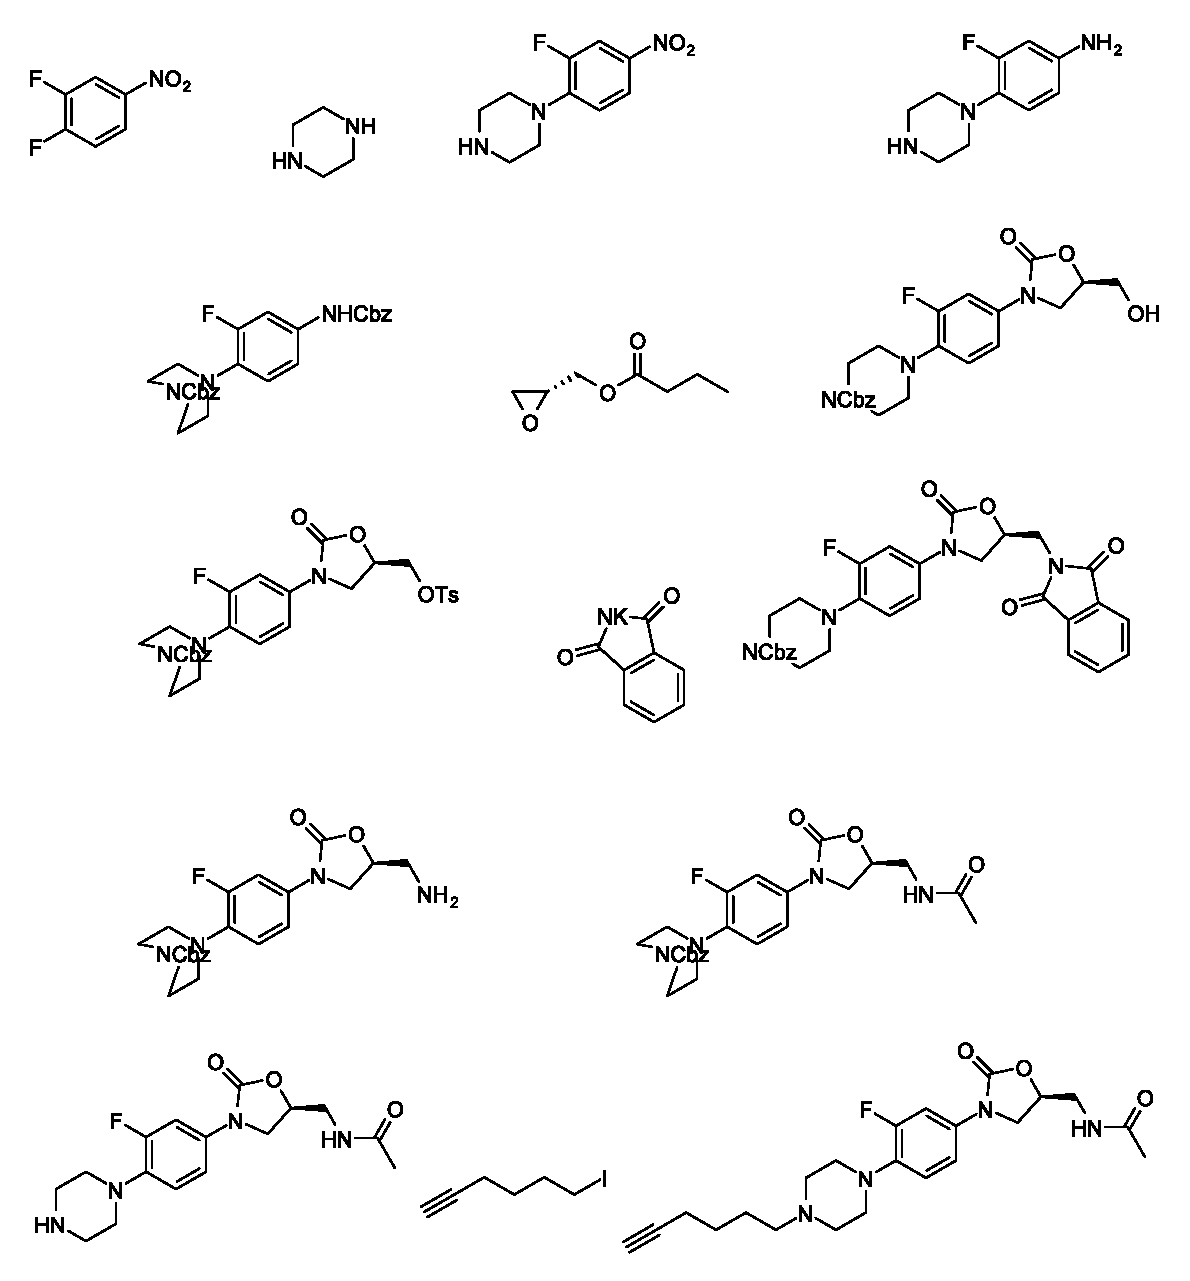
\includegraphics[width=\textwidth]{YLin_synth}
		\caption{Proposed synthesis of linezolid analogue \compound{cmpd:YLin}\cite{Phetsang2014}.
		a) MeCN, reflux, 3 h. 
		b) \ce{H2}, 10 \% Pd/C, THF, 40 psi, <50 $\ ^{\circ}$C, 1.5 h. 
		c) CbzCl, \ce{Na2CO3}, acetone/\ce{H2O}, 1 h at 5 $\ ^{\circ}$C then 16 h at rt. 
		d) \textit{n}-BuLi, THF, -78 $\ ^{\circ}$C for 1 h then add epoxide then -78 $\ ^{\circ}$C for 1.5 h then rt for 3.5 h. 
		e) TsCl, \ce{NEt3}, \ce{CH2Cl2}, 0 $\ ^{\circ}$C for 1.5 h then rt for 3 h. 
		f) MeCN/\ce{H2O}, reflux, 48 h. 
		g) \ce{MeNH2}, EtOH/\ce{H2O}, reflux, 5.5 h. 
		h) \ce{Ac2O}, pyridine, 0 $\ ^{\circ}$C to rt. 
		i) \ce{H2}, 10 \% Pd/C, MeOH/\ce{CH2Cl2}, 1 atm, rt, 16 h. 
		j) \ce{NEt3}, EtOH, reflux.%, 6 h.
		\label{sch:YLin_synth}}
	\end{center}
\end{scheme}

\section{Triazole-linked autoinducer-antibiotic conjugates}

\begin{scheme}[H]
	\begin{center}
		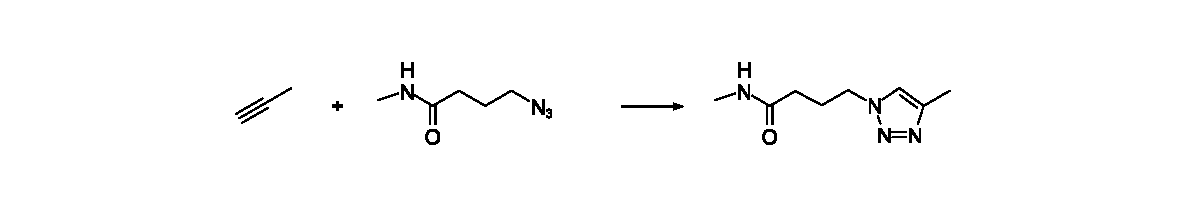
\includegraphics[width=\textwidth]{triazole_synth}
		\caption{\label{sch:}}
	\end{center}
\end{scheme}

\subsection{Synthesis of autoinducers-antibiotic conjugate \compound{cmpd:HL2N3hexpipcip}}

Test reactions using C$_4$-HSL analogue \compound{cmpd:HL2N3} and ciprofloxacin analogue \compound{cmpd:hexpipcip} were performed to find conditions for the click reactions between the azido autoinducers and the alkynyl antibiotics (see \ref{sch:HL2N3hexpipcip_synth} and \ref{tbl:HL2N3hexpipcip_opt}). Stirring at r.t. had no effect even with an extended reaction time. Heating to 50 $^{\circ}$C did lead to slow formation of the product, but a mixture of the 1,4 \compound{cmpd:HL2T4Cip} and 1,5 \compound{cmpd:15HL2T4Cip} isomers was observed \marginnote{check and include ratio from NMR?}. Use of the ligand tris[(1-benzyl-\textit{1H}-1,2,3-triazol-4-yl)methyl]amine (TBTA) \compound{cmpd:TBTA} lead to some conversion at room temperature, however the reaction stopped before completion, probably due to oxidation of the Cu(I) catalytic species. When degassed solvent and an argon atmosphere were used the reaction proceeded to completion at room temperature in around 3 h.

\marginnote{TBTA diagram, isomers diagram}

\renewcommand{\arraystretch}{1.2}
\begin{table}[ht]
  \centering
\begin{tabular}{|p{0.3\textwidth}|p{0.3\textwidth}|}
\hline 
\textbf{Conditions} & \textbf{Outcome} \\ 
\hline 
\ce{CuSO4}$\cdot$\ce{H2O}, sodium ascorbate, \ce{H2O}, \textit{t}-BuOH, air, r.t., 7 d. & No reaction \\ 
\hline 
\ce{CuSO4}$\cdot$\ce{H2O}, sodium ascorbate, \ce{H2O}, \textit{t}-BuOH, air, 50 $^{\circ}$C, 5 d. & 1,3-Triazole product \compound{cmpd:HL2N3hexpipcip} and 1,5 triazole impurity \compound{cmpd:15HL2N3hexpipcip} \\ 
\hline 
\ce{CuSO4}$\cdot$\ce{H2O}, sodium ascorbate, TBTA, \ce{H2O}, \textit{t}-BuOH, air, r.t., 3 h. & 1,3-Triazole product \compound{cmpd:HL2N3hexpipcip} and starting materials \compound{cmpd:HL2N3} and  \compound{cmpd:hexpipcip}\\ 
\hline 
\ce{CuSO4}$\cdot$\ce{H2O}, sodium ascorbate, TBTA, \ce{H2O}, \textit{t}-BuOH, Ar, r.t., 3 h. & 1,3-Triazole product \compound{cmpd:HL2N3hexpipcip} \\ 
\hline 
\end{tabular}
\caption{Conditions attempted for the synthesis of \compound{cmpd:HL2N3hexpipcip} (see \ref{sch:HL2N3hexpipcip_synth}).\label{tbl:HL2N3hexpipcip_opt}} 
\end{table}

\begin{scheme}[H]
	\begin{center}
		\schemeref[HL2N3]{cmpd:HL2N3}
		\schemeref[hexpipcip]{cmpd:hexpipcip}
		\schemeref[HL2N3hexpipcip]{cmpd:HL2N3hexpipcip}
		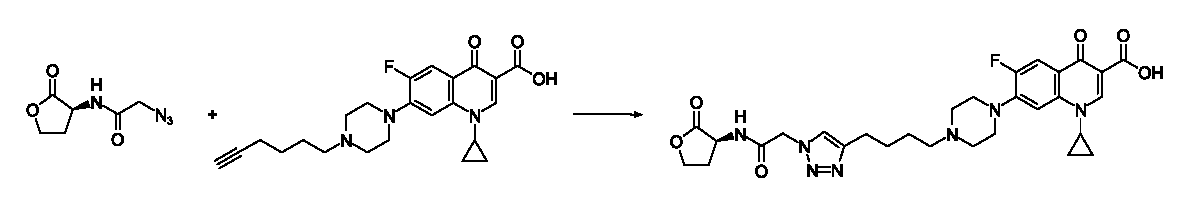
\includegraphics[width=\textwidth]{HL2N3hexpipcip_synth}
		\caption{Synthesis of \compound{cmpd:HL2N3hexpipcip}. a) see \ref{tbl:HL2N3hexpipcip_opt}. \label{sch:HL2N3hexpipcip_synth}}
	\end{center}
\end{scheme}

\subsection{Synthesis of first triazole-linked library}

\section{Biological testing - Round 1}

Insert here

\section{Autoinducer analogue-ciprofloxacin conjugates}

Talk about precedent set by Ganguly.
Better against mature biofilms
%Is it just more lipophillic?

\begin{scheme}[H]
	\begin{center}
		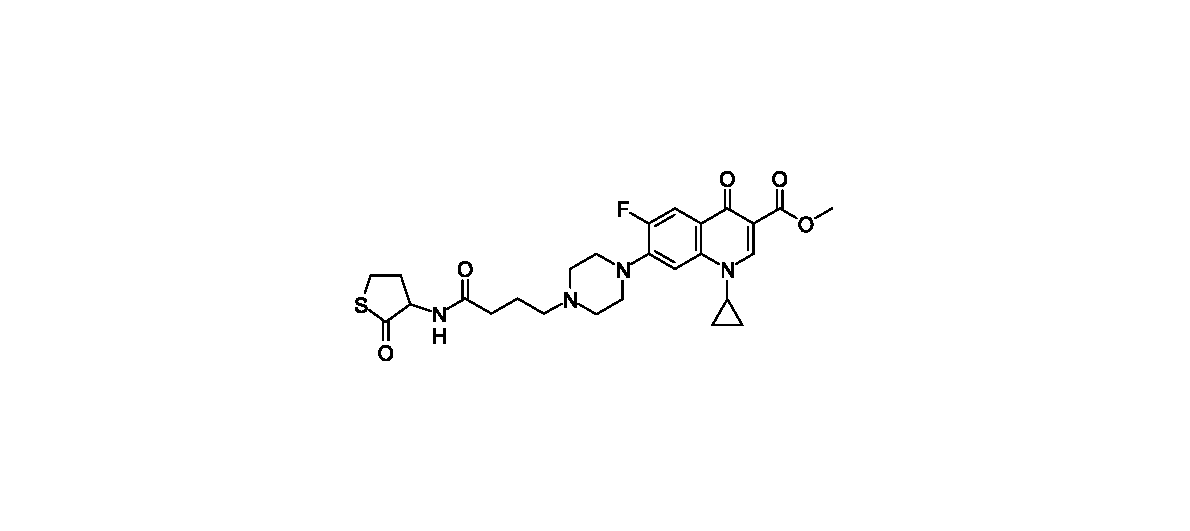
\includegraphics[width=\textwidth]{SHL4CipMe}
		\caption{\label{sch:}}
	\end{center}
\end{scheme}

\begin{scheme}[H]
	\begin{center}
		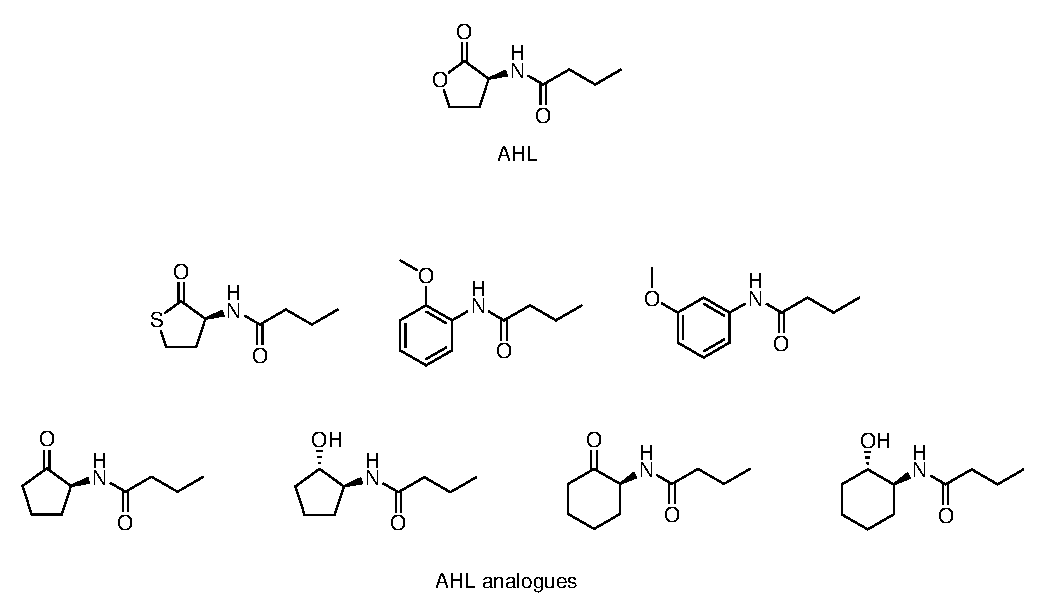
\includegraphics[width=\textwidth]{AHL_analogues}
		\caption{\label{sch:}}
	\end{center}
\end{scheme}

Introduce initial strategy of making bromide then azide, and diverting down the two different paths to make directly linked or triazole linked products.

\begin{scheme}[H]
	\begin{center}
		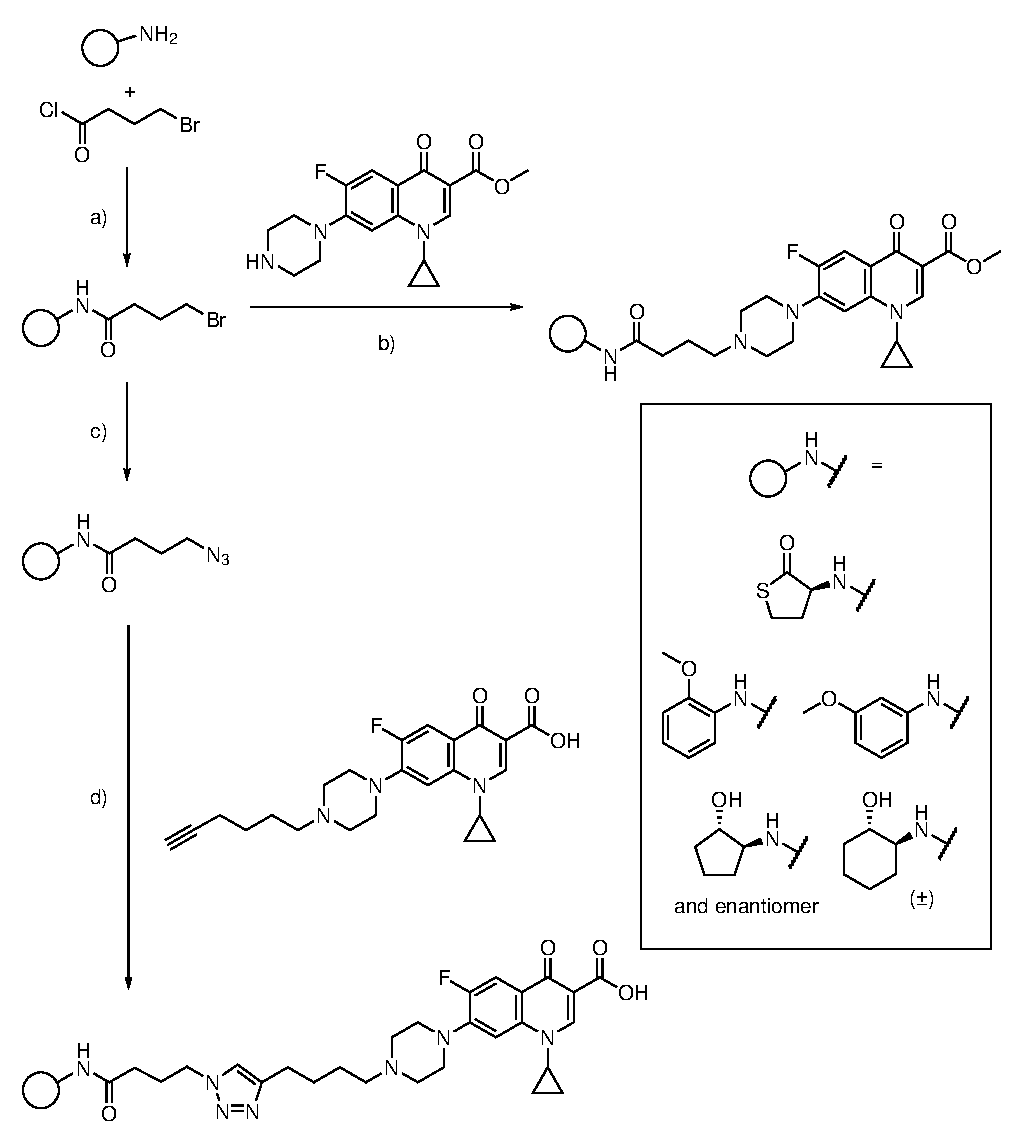
\includegraphics[width=\textwidth]{branching_synth_general}
		\caption{\label{sch:}}
	\end{center}
\end{scheme}

%\subsubsection{Amine-linked autoinducer analogue-antibiotic conjugates}

%\subsubsection{Triazole-linked autoinducer analogue-antibiotic conjugates}

\subsection{Sulfur AHL derivatives}

\begin{scheme}[H]
	\begin{center}
		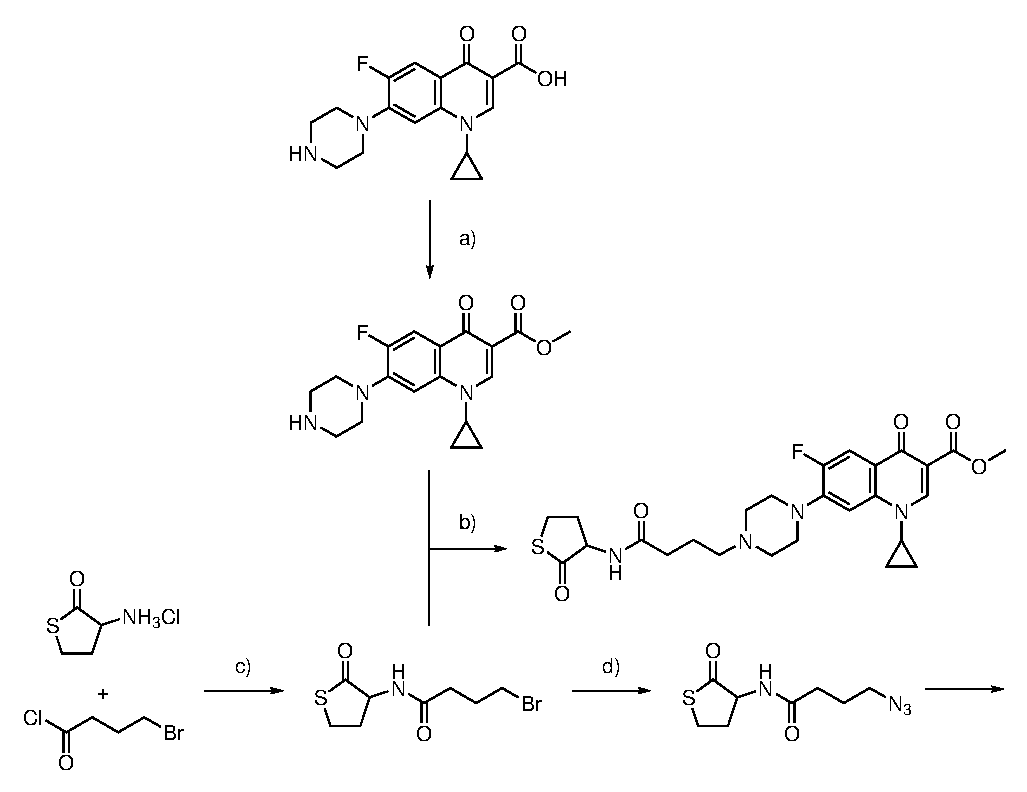
\includegraphics[width=\textwidth]{SHL_synth}
		\caption{a) pTSA, MeOH, 72 h, reflux, 83.3 \%, ~ 8 g, LMO-2-015, LMO-2-016
			b) K2CO3, MeCN, reflux, 24 h, 12.2 \%, ~ 20 g, LMO-2-017, LMO-2-021
			c) NaHCO3, DCM, H2O, 0 oC, 1 h 87.9 \% ~ 0.5 g, LMO-2-013, LMO-2-014
			d) NaN3, MeCN, 80 oC, 1.5 h, 89.3 \%, ? g, LMO-2-018, LMO-2-019, LMO-2-020\label{sch:}}
	\end{center}
\end{scheme}

\begin{scheme}[H]
	\begin{center}
		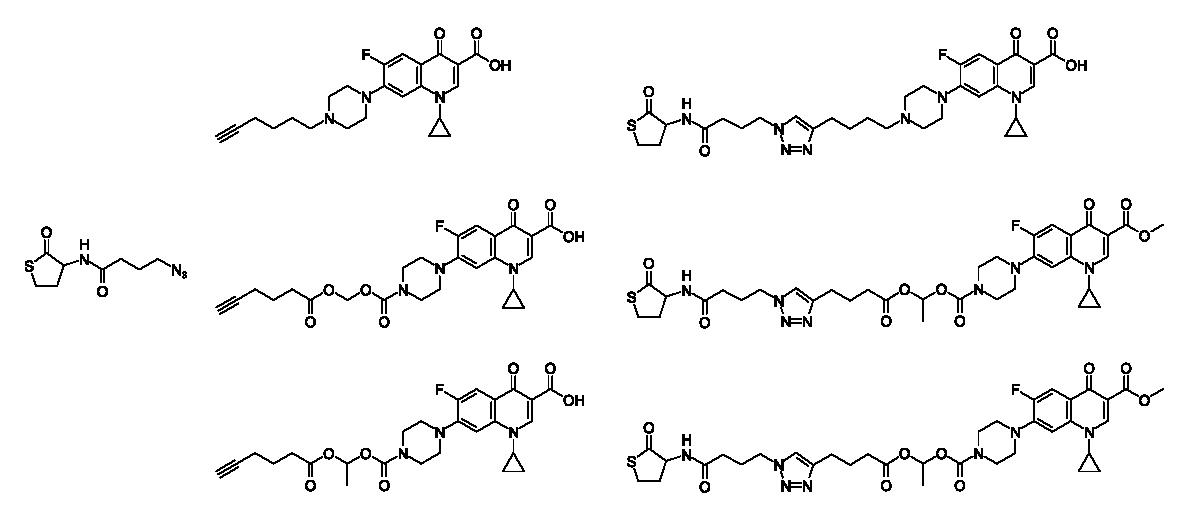
\includegraphics[width=\textwidth]{SHL_finals_synth}
		\caption{a) CuI, DIPEA, DCM, Ar, r.t., 1 d, ? \%, LMO-2-022, went to completion after adding more CuI.
			b) CuI, DIPEA, DCM, Ar, r.t., 1 d, ? \%, LMO-2-023, didn't go to completion, columned anyway.
			c) CuI, DIPEA, DCM, Ar, r.t., 1 d, LMO-2-024, didn't go to completion
			OR CuSO4, NaAsc, THPTA, H2O, tBuOH, r.t., 1.5 d, LMO-2-027, went to completion but too little recovered for NMR\label{sch:}}
	\end{center}
\end{scheme}


\subsection{2-methoxyphenyl derivatives}

\begin{scheme}[H]
	\begin{center}
		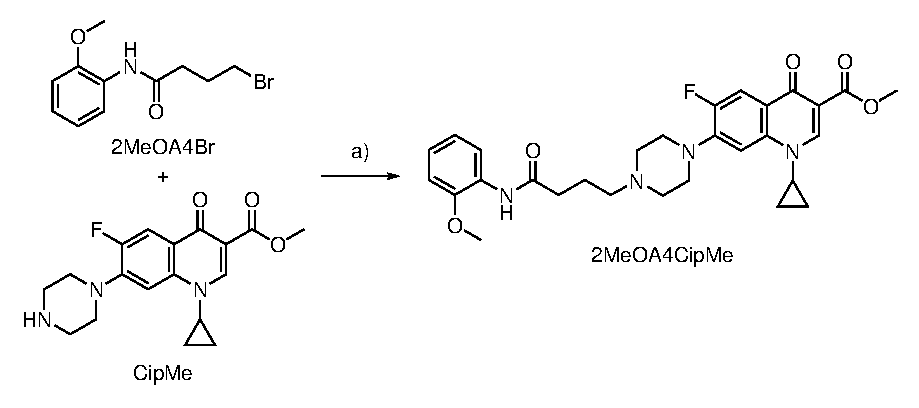
\includegraphics[width=\textwidth]{2MeOA4_synth}
		\caption{\label{sch:}}
	\end{center}
\end{scheme}

\begin{scheme}[H]
	\begin{center}
		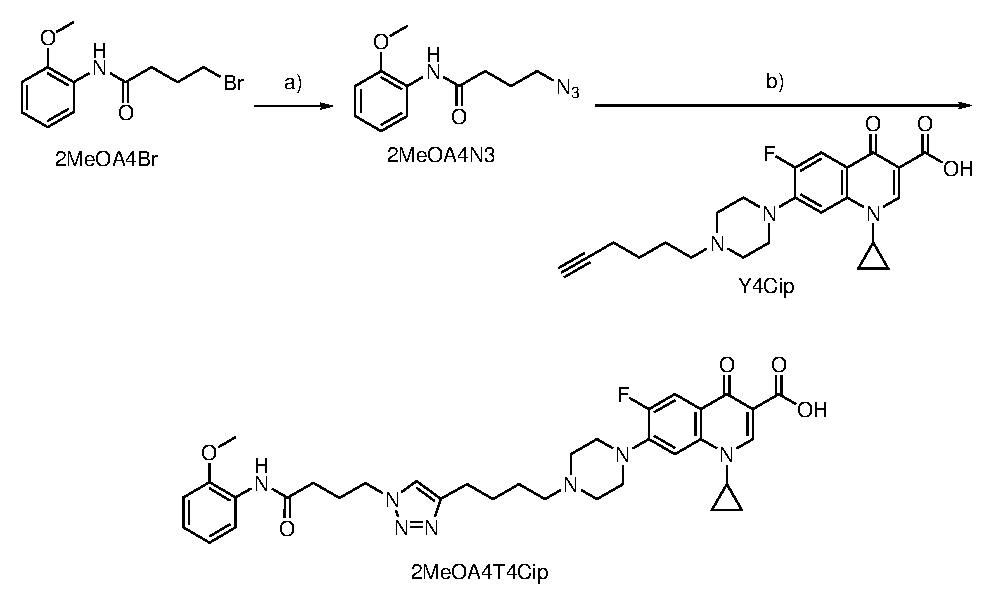
\includegraphics[width=\textwidth]{2MeOA4T4Cip_synth}
		\caption{\label{sch:}}
	\end{center}
\end{scheme}

\subsection{3-methoxyphenyl derivatives}

\begin{scheme}[H]
	\begin{center}
		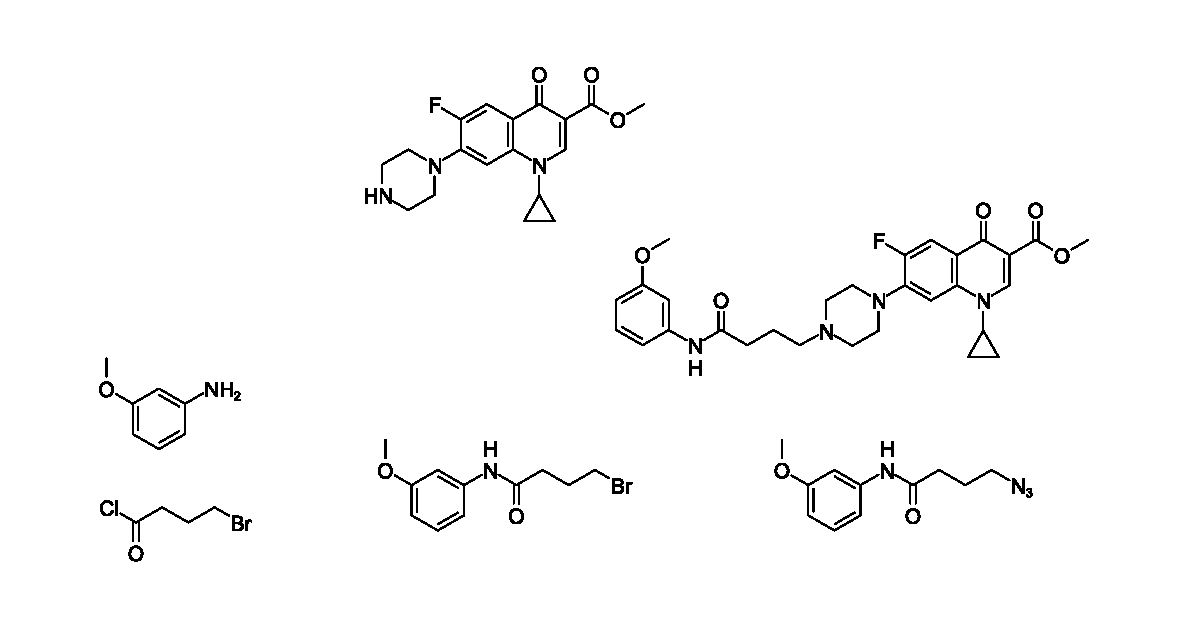
\includegraphics[width=\textwidth]{3MeOA4_synth}
		\caption{\label{sch:}}
	\end{center}
\end{scheme}

\begin{scheme}[H]
	\begin{center}
		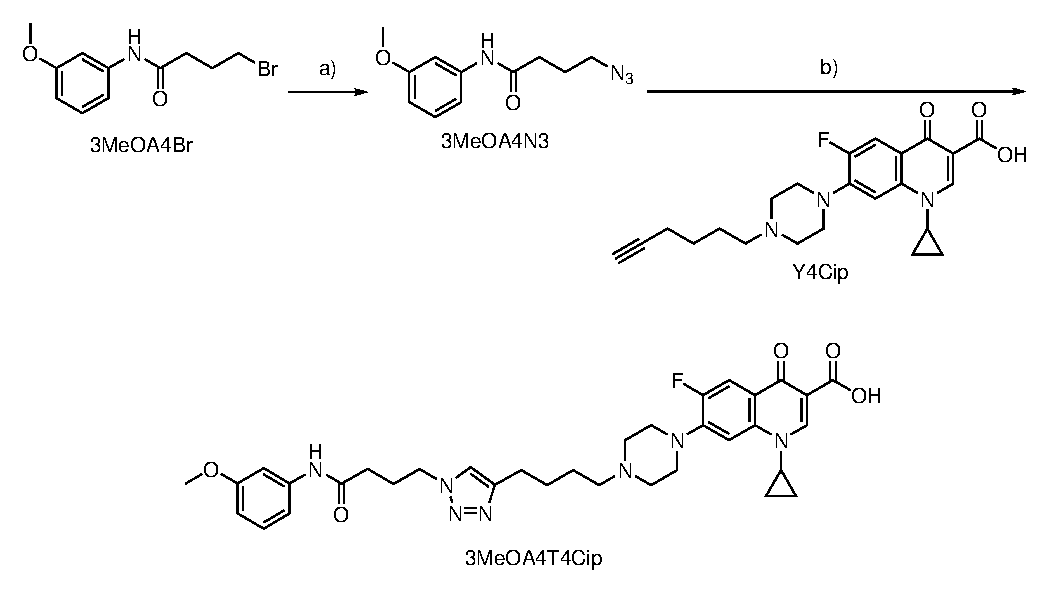
\includegraphics[width=\textwidth]{3MeOA4T4Cip_synth}
		\caption{\label{sch:}}
	\end{center}
\end{scheme}

\subsection{Cyclopentyl alcohol derivatives}

\subsubsection{Head-group synthesis}

\begin{scheme}[H]
	\begin{center}
		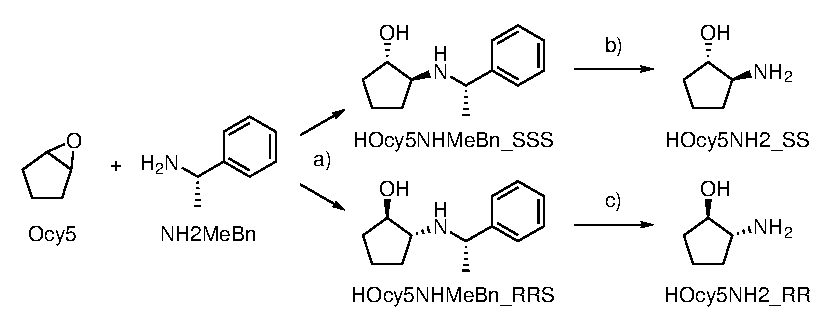
\includegraphics[width=\textwidth]{HOcy5NH2_synth}
		\caption{a) AlMe3, DCM, 0 oC. 32.1 \%(LMO-2-053, SSS), 35.2 \% (LMO-2-053, RRS)
			b) Pd(OH)2, MeOH, H2, 5 atm, 1 day, 100 \% (LMO-2-061, SSS), 100 \% (LMO-2-057, LMO-2-059 RRS)\label{sch:}}
	\end{center}
\end{scheme}

\subsubsection{Initial branching strategy}

Failed. Lots of side-products.

\begin{scheme}[H]
	\begin{center}
		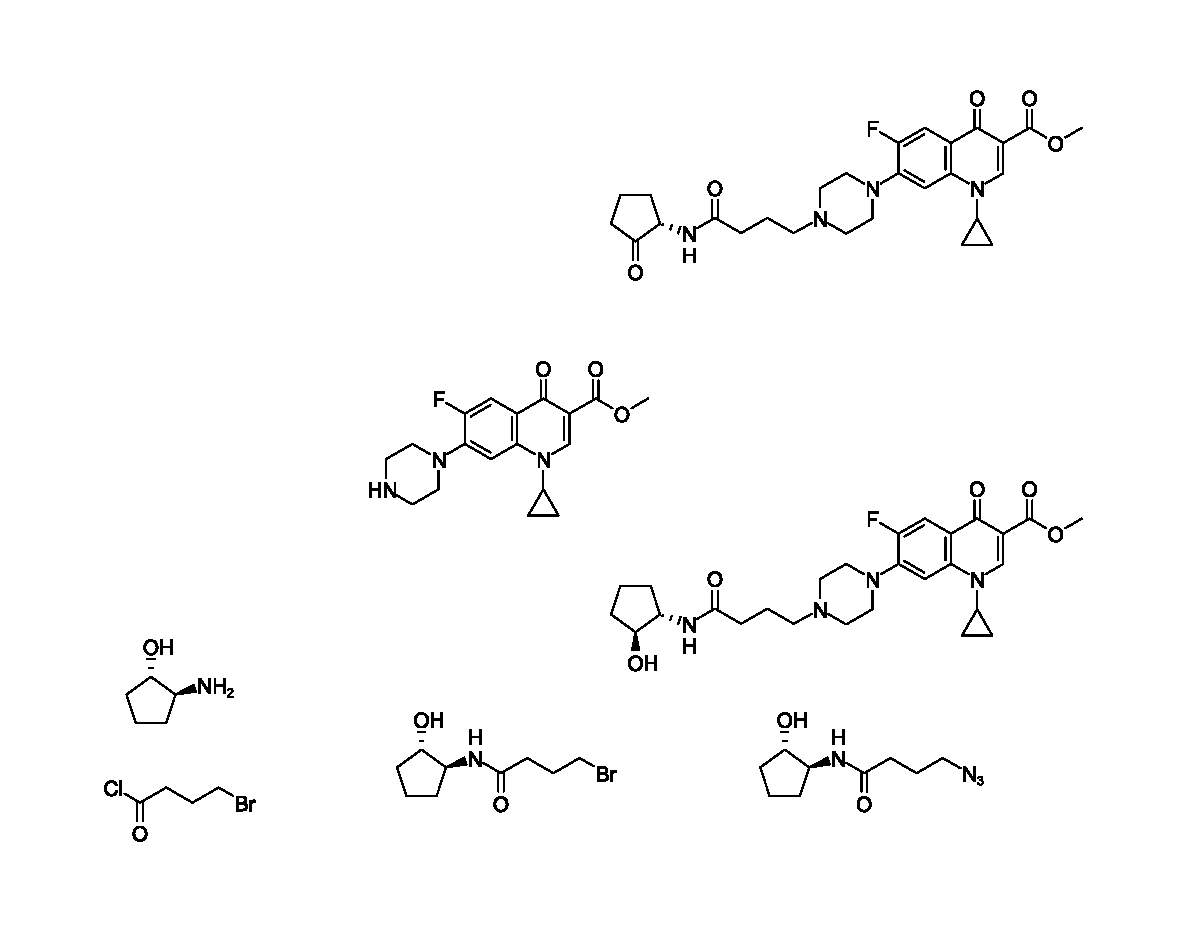
\includegraphics[width=\textwidth]{HOcy5NH4_synth_A}
		\caption{\label{sch:}}
	\end{center}
\end{scheme}

\subsubsection{TBS protection strategy}

Want to protect alcohol to stop side reactions

\begin{scheme}[H]
	\begin{center}
		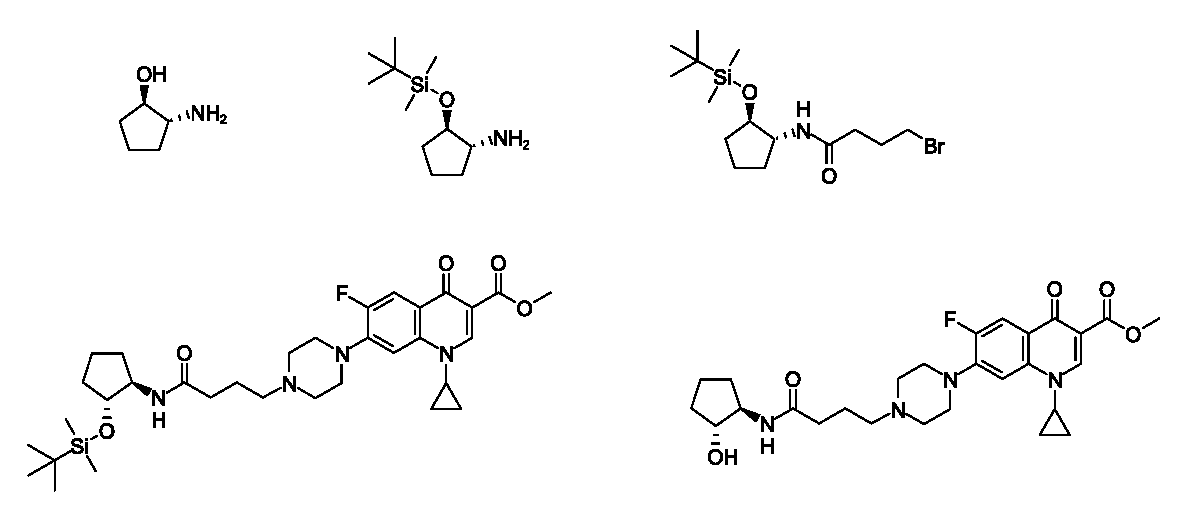
\includegraphics[width=\textwidth]{HOcy5NH4_synth_B}
		\caption{\label{sch:}}
	\end{center}
\end{scheme}

Protection optimisation

Still get side-reactions when adding tail

\subsubsection{Attaching the linker to ciprofloxacin first}

Given the side-reactions and low yields associated with the literate synthesis of the S$_N$2 conjugates proposed by Ganguly et. al\cite{Ganguly2011}, we investigated a second synthesis, building up the linker on the ciprofloxacin side before coupling with the head group (see \ref{sch:HOcy5NH4CipMeRR_synth}).

\subsubsubsection{Synthesis of methyl-protected ciprofloxacin with linker with terminal carboxylate}

\begin{scheme}[H]
	\begin{center}
		\schemeref[CipMe]{cmpd:CipMe}
		\schemeref[tBu4Br]{cmpd:tBu4Br}
		\schemeref[tBu4CipMe]{cmpd:tBu4CipMe}
		\schemeref[4CipMe]{cmpd:4CipMe}
		\schemeref[HOcy5NH4CipMe]{cmpd:HOcy5NH4CipMe}
		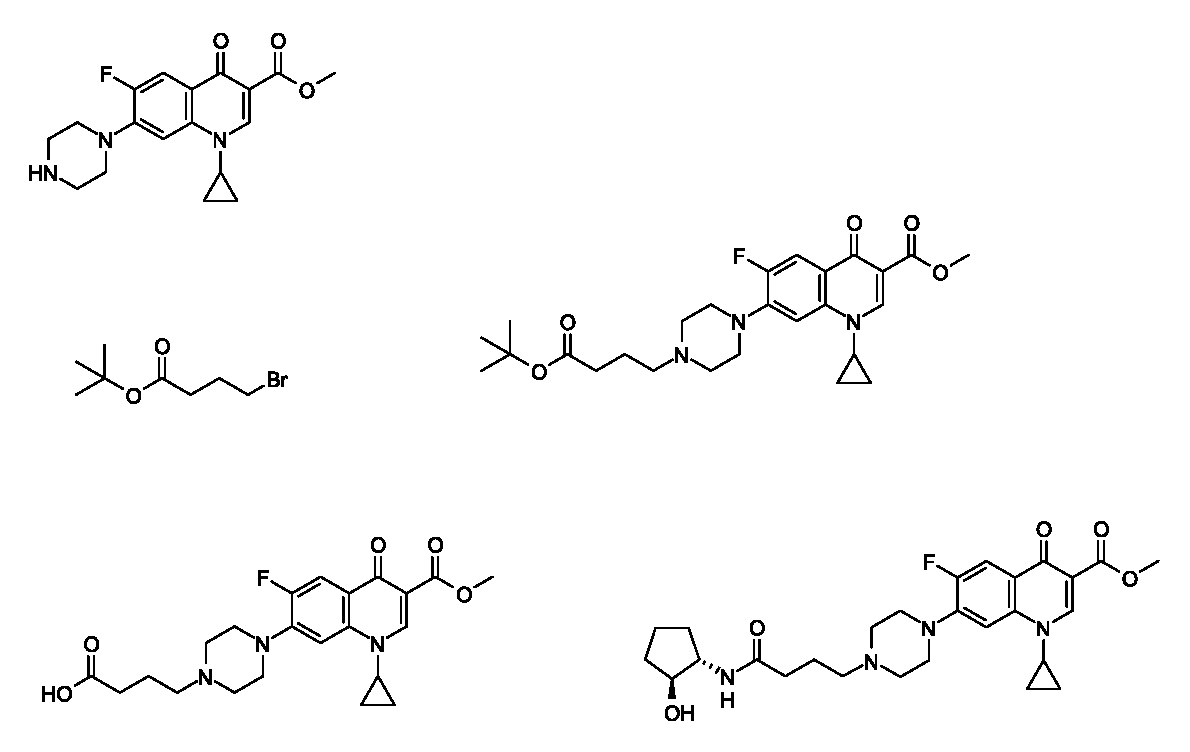
\includegraphics[width=\textwidth]{HOcy5NH4CipMeRR_synth}
		\caption{Synthesis of \compound{cmpd:HOcy5NH4CipMeRR}. 
			a) . 
			\label{sch:HOcy5NH4CipMeRR_synth}}
	\end{center}
\end{scheme}

\subsubsection{Triazoles by two-step reaction}
Talk about moving to two-step reaction.

\begin{scheme}[H]
	\begin{center}
		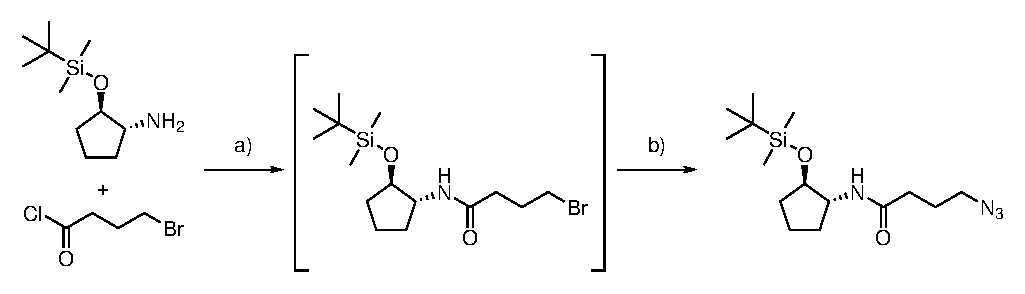
\includegraphics[width=\textwidth]{TBSOcy5NH4N3_synth_2step}
		\caption{\label{sch:}}
	\end{center}
\end{scheme}

Did click, then failed to deprotect.

\subsubsection{Triazoles from the chloride}

\begin{scheme}[H]
	\begin{center}
		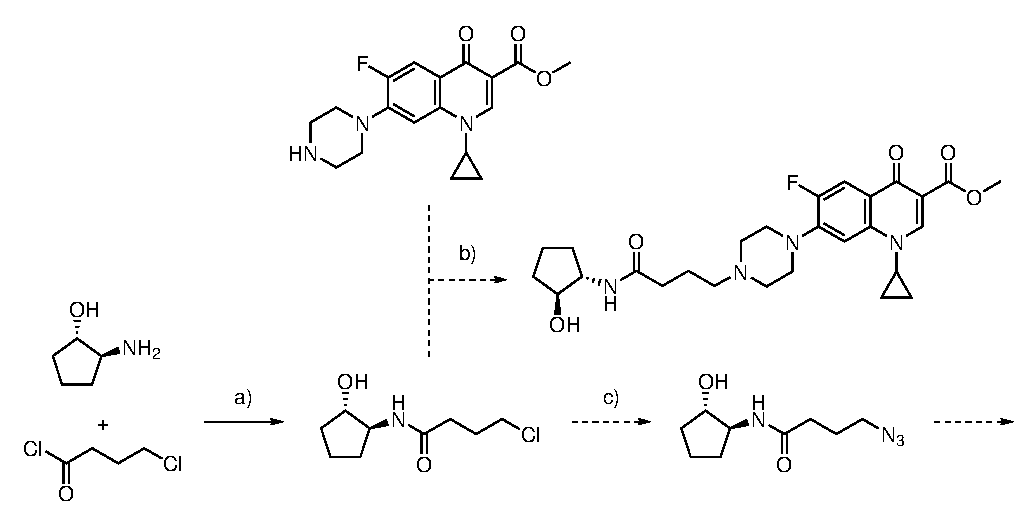
\includegraphics[width=\textwidth]{HOcy5NH4_synth_C}
		\caption{\label{sch:}}
	\end{center}
\end{scheme}

\begin{scheme}[H]
	\begin{center}
		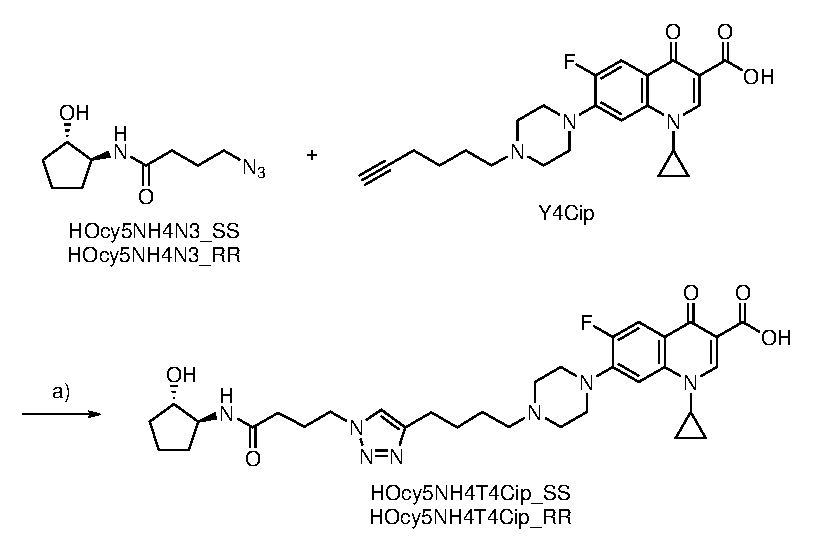
\includegraphics[width=\textwidth]{HOcy5NH4T4Cip_synth}
		\caption{\label{sch:}}
	\end{center}
\end{scheme}

This worked.

\subsection{Cyclohexyl alcohol derivatives}
%\subsubsection{Other head groups}
%Inc. negative controls

\section{Biological testing - Round 2}

To be done
